% QuickEIP Programming and Implementation Manual
% Copyright (c) 2026 Adam G. Sweeney. Text written to ASD-STE100 and edited
% to The Chicago Manual of Style, 18th edition.
%
% Build (Tectonic, XeTeX engine):  tectonic quickeip-manual.tex
% QuickEIP Programming and Implementation Manual: shared preamble.
% Build: tectonic quickeip-manual.tex
\documentclass[11pt,twoside,openright]{book}

\usepackage[letterpaper,inner=1.15in,outer=1in,top=1in,bottom=1.05in,
            headheight=14pt,headsep=0.3in]{geometry}

% ---- fonts (XeTeX through Tectonic) ---------------------------------------
\usepackage{fontspec}
\usepackage{unicode-math}
\setmainfont{texgyrepagella}[
  Extension=.otf, UprightFont=*-regular, BoldFont=*-bold,
  ItalicFont=*-italic, BoldItalicFont=*-bolditalic, Ligatures=TeX]
\setsansfont{texgyreheros}[
  Extension=.otf, UprightFont=*-regular, BoldFont=*-bold,
  ItalicFont=*-italic, BoldItalicFont=*-bolditalic, Ligatures=TeX]
\setmonofont{DejaVuSansMono}[
  Extension=.ttf, UprightFont=*, BoldFont=*-Bold,
  ItalicFont=*-Oblique, BoldItalicFont=*-BoldOblique, Scale=0.84]
\setmathfont{texgyrepagella-math.otf}

\usepackage{microtype}
% Code words cannot hyphenate; let a line stretch instead of overflowing.
\setlength{\emergencystretch}{3em}

% ---- color, boxes, figures ------------------------------------------------
\usepackage{xcolor}
\definecolor{navy}{HTML}{1B2F4B}
\definecolor{steel}{HTML}{3D5A80}
\definecolor{teal}{HTML}{2A9D8F}
\definecolor{amber}{HTML}{C77700}
\definecolor{signal}{HTML}{B3261E}
\definecolor{noteblue}{HTML}{1F6FB2}
\definecolor{codebg}{HTML}{F5F7FA}
\definecolor{rulegray}{HTML}{C9D1DB}
\definecolor{commentgreen}{HTML}{4E7A55}
\definecolor{stringred}{HTML}{9A3324}

\usepackage{graphicx}
\usepackage{tikz}
\usetikzlibrary{positioning,arrows.meta,shapes.geometric,shapes.misc,calc,fit,backgrounds,decorations.pathreplacing}
\usepackage[most]{tcolorbox}

% ---- tables and lists -----------------------------------------------------
\usepackage{booktabs}
\usepackage{tabularx}
\usepackage{longtable}
\usepackage{array}
\usepackage{multicol}
\usepackage[shortlabels]{enumitem}
\newcolumntype{L}{>{\raggedright\arraybackslash}X}
\newcolumntype{P}[1]{>{\raggedright\arraybackslash}p{#1}}
\renewcommand{\arraystretch}{1.18}
\setlength{\tabcolsep}{5pt}
\setlist{itemsep=2pt,topsep=4pt}
\setlist[enumerate,1]{label=\arabic*.,leftmargin=*}

% ---- captions: Chicago style, label then period ---------------------------
\usepackage[font={small},labelfont={bf,sf},labelsep=period,
            justification=raggedright,singlelinecheck=false]{caption}
\captionsetup[table]{position=top,skip=4pt}
\captionsetup[figure]{position=bottom,skip=6pt}

% ---- headings -------------------------------------------------------------
\usepackage{titlesec}
\titleformat{\chapter}[display]
  {\sffamily\bfseries\color{navy}}
  {\normalsize\mdseries\scshape\color{steel}\chaptertitlename\ \thechapter}
  {4pt}
  {\Huge\raggedright}
  [\vspace{4pt}{\color{teal}\titlerule[1.2pt]}]
\titlespacing*{\chapter}{0pt}{-10pt}{26pt}
\titleformat{\section}{\sffamily\Large\bfseries\color{navy}}{\thesection}{0.7em}{}
\titleformat{\subsection}{\sffamily\large\bfseries\color{steel}}{\thesubsection}{0.7em}{}
\titleformat{\subsubsection}{\sffamily\normalsize\bfseries\color{steel}}{}{0em}{}
\titlespacing*{\section}{0pt}{16pt}{6pt}
\titlespacing*{\subsection}{0pt}{12pt}{4pt}
\titlespacing*{\subsubsection}{0pt}{10pt}{3pt}
\setcounter{secnumdepth}{2}
\setcounter{tocdepth}{1}

% ---- running heads --------------------------------------------------------
\usepackage{fancyhdr}
\pagestyle{fancy}
\fancyhf{}
\renewcommand{\headrulewidth}{0.4pt}
\renewcommand{\headrule}{{\color{rulegray}\hrule height\headrulewidth width\headwidth}}
\fancyhead[LE]{\sffamily\small\color{steel}\leftmark}
\fancyhead[RO]{\sffamily\small\color{steel}\rightmark}
\fancyfoot[LE,RO]{\sffamily\small\thepage}
\fancyfoot[RE,LO]{\sffamily\scriptsize\color{steel}QuickEIP Programming and Implementation Manual}
\renewcommand{\chaptermark}[1]{\markboth{\thechapter.\ #1}{}}
\renewcommand{\sectionmark}[1]{\markright{\thesection\ \ #1}}
\fancypagestyle{plain}{\fancyhf{}\renewcommand{\headrulewidth}{0pt}%
  \renewcommand{\headrule}{}\fancyfoot[LE,RO]{\sffamily\small\thepage}}

% ---- code listings --------------------------------------------------------
\usepackage{listings}
\lstdefinestyle{qe}{
  basicstyle=\ttfamily\small,
  keywordstyle=\color{navy}\bfseries,
  commentstyle=\color{commentgreen}\itshape,
  stringstyle=\color{stringred},
  backgroundcolor=\color{codebg},
  frame=leftline, framerule=2.5pt, rulecolor=\color{teal},
  xleftmargin=10pt, framexleftmargin=6pt, framesep=4pt,
  aboveskip=8pt, belowskip=8pt,
  columns=fullflexible, keepspaces=true, showstringspaces=false,
  breaklines=true, breakatwhitespace=true,
  upquote=true, tabsize=4,
}
\lstset{style=qe,language=C}
\lstdefinelanguage{shell}{morecomment=[l]{\#},sensitive=true}
\lstdefinelanguage{cmake}{
  morekeywords={cmake_minimum_required,project,list,include,add_subdirectory,
    add_executable,target_link_libraries,set,idf_component_register,
    idf_build_set_property,APPEND,PRIVATE,CACHE,BOOL,VERSION,SRCS,INCLUDE_DIRS,REQUIRES},
  morecomment=[l]{\#},morestring=[b]",sensitive=true}
\lstdefinelanguage{make}{morekeywords={include},morecomment=[l]{\#},sensitive=true}
\lstdefinelanguage{eds}{morecomment=[l]{\$},morestring=[b]",sensitive=true}
\lstdefinelanguage{yaml}{morecomment=[l]{\#},sensitive=true}

% ---- admonitions (ASD-STE100: warning, caution, note) ---------------------
\newtcolorbox{warning}{enhanced,breakable,colback=signal!5,colframe=signal,
  boxrule=0.8pt,arc=1.5pt,left=8pt,right=8pt,top=4pt,bottom=4pt,
  fonttitle=\sffamily\bfseries,coltitle=white,
  title={\raisebox{-1pt}{\large$\triangle$}\ \ WARNING}}
\newtcolorbox{caution}{enhanced,breakable,colback=amber!6,colframe=amber,
  boxrule=0.8pt,arc=1.5pt,left=8pt,right=8pt,top=4pt,bottom=4pt,
  fonttitle=\sffamily\bfseries,coltitle=white,title={CAUTION}}
\newtcolorbox{note}{enhanced,breakable,colback=noteblue!5,colframe=noteblue!80,
  boxrule=0pt,leftrule=3pt,arc=0pt,left=8pt,right=8pt,top=4pt,bottom=4pt,
  fontupper=\small}
\newcommand{\notelabel}{\textsf{\textbf{\color{noteblue}NOTE:}}\ }

% Procedure: a titled, numbered task (ASD-STE100 procedural writing).
\newtcolorbox{procedure}[1]{enhanced,breakable,colback=white,colframe=steel,
  boxrule=0.6pt,arc=1.5pt,left=6pt,right=8pt,top=4pt,bottom=4pt,
  fonttitle=\sffamily\bfseries\small,colbacktitle=steel!12,coltitle=navy,
  title={Procedure: #1}}

% API entry: name, then the prototype in a shaded box.
\newtcolorbox{protobox}{enhanced,colback=codebg,colframe=rulegray,boxrule=0.4pt,
  arc=1pt,left=6pt,right=6pt,top=3pt,bottom=3pt,before skip=3pt,after skip=4pt,
  fontupper=\ttfamily\small}
% Label keys must not contain an active underscore: the aux file of an
% \include'd chapter is read back after the underscore package activates it.
\ExplSyntaxOn
\str_new:N \l_qe_key_str
\cs_new_protected:Npn \qe_setkey:n #1
  { \str_set:Nn \l_qe_key_str {#1} \str_replace_all:Nnn \l_qe_key_str { _ } { - } }
\NewDocumentCommand{\apilabel}{m}{ \qe_setkey:n {#1} \exp_args:Nx \label { api: \l_qe_key_str } }
\NewDocumentCommand{\apipageref}{m}{ \qe_setkey:n {#1} \exp_args:Nx \pageref { api: \l_qe_key_str } }
\ExplSyntaxOff
\newcommand{\api}[2]{%
  \par\addvspace{10pt}\needspace{6\baselineskip}%
  \phantomsection\apilabel{#1}%
  \noindent{\sffamily\bfseries\color{navy}#1}\par\nopagebreak
  \begin{protobox}\raggedright #2\end{protobox}\nopagebreak}
\newcommand{\apiidx}[1]{\noindent\texttt{#1}\dotfill\apipageref{#1}\par}
\usepackage{needspace}

% ---- inline helpers -------------------------------------------------------
\newcommand{\code}[1]{\texttt{#1}}
\newcommand{\file}[1]{\texttt{#1}}
% Direction arrows that work in text and in math (subscripts of equations).
\DeclareRobustCommand{\OT}{\ifmmode\text{O}{\to}\text{T}\else O\kern0.05em$\to$\kern0.05em T\fi}
\DeclareRobustCommand{\TO}{\ifmmode\text{T}{\to}\text{O}\else T\kern0.05em$\to$\kern0.05em O\fi}
\newcommand{\hex}[1]{\texttt{0x#1}}
\newcommand{\term}[1]{\textit{#1}}
\newcommand{\menu}[1]{\textsf{#1}}

\usepackage{amsmath}
\usepackage{siunitx}
\sisetup{group-separator={,},group-minimum-digits=4}

% ---- links last -----------------------------------------------------------
\usepackage[hidelinks,bookmarksnumbered,pdfusetitle]{hyperref}
\hypersetup{pdftitle={QuickEIP Programming and Implementation Manual},
  pdfauthor={Adam G. Sweeney},pdfsubject={EtherNet/IP scanner and adapter stack},
  pdfkeywords={EtherNet/IP, CIP, embedded, C99, QuickEIP}}
\usepackage{bookmark}

% Load last: an active underscore breaks PGF if it loads first.
\usepackage[strings,nohyphen]{underscore}


\newcommand{\docnumber}{QE-PIM-200}
\newcommand{\docrevision}{Revision A}
\newcommand{\swversion}{2.0.0}
\newcommand{\docdate}{November 2026}

\begin{document}

% =========================================================================
% Cover / title page
% =========================================================================
\frontmatter
\pagestyle{empty}
\begin{titlepage}
\begin{tikzpicture}[remember picture,overlay]
  % background bands
  \fill[navy] (current page.north west) rectangle ([yshift=-15.2cm]current page.north east);
  \fill[teal] ([yshift=-15.2cm]current page.north west) rectangle ([yshift=-15.55cm]current page.north east);
  \fill[steel!10] ([yshift=-15.55cm]current page.north west) rectangle (current page.south east);

  % network motif: a scanner node linked to adapter nodes
  \begin{scope}[shift={([xshift=-6.4cm,yshift=-7.6cm]current page.north east)}]
    \foreach \a/\r in {20/3.4,60/2.6,105/3.1,150/2.4,200/3.3,245/2.7,290/3.2,335/2.5}{
      \draw[white!45!navy,line width=0.8pt] (0,0) -- (\a:\r);
      \fill[teal] (\a:\r) circle (4.2pt);
      \fill[navy] (\a:\r) circle (1.8pt);
    }
    \foreach \a/\b in {20/60,105/150,200/245,290/335}{
      \draw[white!30!navy,line width=0.5pt,dashed] (\a:3.0) -- (\b:2.5);
    }
    \draw[teal,line width=1.2pt] (0,0) circle (1.25cm);
    \draw[white!35!navy,line width=0.6pt] (0,0) circle (4.1cm);
    \fill[white] (0,0) circle (0.78cm);
    \node[navy,font=\sffamily\bfseries\small,align=center] at (0,0) {CIP};
  \end{scope}

  % title block
  \node[anchor=north west,text=teal!70!white,font=\sffamily\bfseries\large]
    at ([xshift=2.2cm,yshift=-3.0cm]current page.north west)
    {ETHERNET/IP SCANNER AND ADAPTER STACK};
  \node[anchor=north west,text=white,font=\sffamily\bfseries\fontsize{58}{60}\selectfont]
    at ([xshift=2.1cm,yshift=-3.9cm]current page.north west) {QuickEIP};
  \node[anchor=north west,text=white,font=\sffamily\fontsize{22}{27}\selectfont,align=left]
    at ([xshift=2.2cm,yshift=-6.6cm]current page.north west)
    {Programming and\\Implementation Manual};
  \node[anchor=north west,text=white!80!steel,font=\sffamily\normalsize,align=left,text width=9cm]
    at ([xshift=2.2cm,yshift=-9.4cm]current page.north west)
    {Portable C99 for embedded targets: NetBurner, ESP32, Teknic ClearCore, Linux, and Windows};
  \node[anchor=south west,text=white,font=\sffamily\small]
    at ([xshift=2.2cm,yshift=-14.6cm]current page.north west)
    {Software version \swversion\quad\textbar\quad \docnumber, \docrevision};

  % author block
  \node[anchor=north west,font=\sffamily\small\color{steel},align=left]
    at ([xshift=2.2cm,yshift=-17.2cm]current page.north west) {AUTHOR AND DEVELOPER};
  \node[anchor=north west,font=\sffamily\bfseries\fontsize{24}{28}\selectfont\color{navy},align=left]
    at ([xshift=2.2cm,yshift=-17.9cm]current page.north west) {Adam G. Sweeney};
  \node[anchor=north west,font=\sffamily\small\color{navy!80},align=left]
    at ([xshift=2.2cm,yshift=-19.2cm]current page.north west) {agsweeney@gmail.com};

  \draw[rulegray,line width=0.6pt]
    ([xshift=2.2cm,yshift=-21.2cm]current page.north west) -- ([xshift=-2.2cm,yshift=-21.2cm]current page.north east);
  \node[anchor=north west,font=\sffamily\footnotesize\color{steel},align=left,text width=8.5cm]
    at ([xshift=2.2cm,yshift=-21.6cm]current page.north west)
    {Written in ASD-STE100 Simplified Technical English.\\
     Edited to \textit{The Chicago Manual of Style}, 18th edition.};
  \node[anchor=north east,font=\sffamily\footnotesize\color{steel},align=right]
    at ([xshift=-2.2cm,yshift=-21.6cm]current page.north east)
    {\docdate\\MIT License};
\end{tikzpicture}
\end{titlepage}

% =========================================================================
% Copyright page (verso)
% =========================================================================
\newpage
\thispagestyle{empty}
\vspace*{\fill}
{\small\raggedright
\textbf{QuickEIP Programming and Implementation Manual}\\
Document \docnumber, \docrevision, \docdate\\
For QuickEIP software version \swversion

\bigskip
Copyright \textcopyright\ 2026 Adam G. Sweeney. All rights reserved.

\medskip
The QuickEIP software is released under the MIT License. The full license
text is in the file \file{LICENSE} at the root of the source repository. The
software is supplied ``as is,'' without warranty of any kind.

\medskip
EtherNet/IP\texttrademark\ and CIP\texttrademark\ are trademarks of ODVA,
Inc. ASD-STE100\textsuperscript{\textregistered} is a trademark of ASD
(AeroSpace, Security and Defence Industries Association of Europe). All other
product names are trademarks of their respective owners. Their use in this
manual identifies products and does not imply endorsement.

\medskip
\textbf{Status of tests.} Each platform section of this manual states what
has been built, what has been run, and what has been tested with a
programmable logic controller (PLC). A successful build does not show that a
port operates on a network. Do the hardware tests in chapter~\ref{ch:porting}
before you use QuickEIP in a product.

\medskip
\textbf{Editorial conventions.} This manual uses ASD-STE100 Simplified
Technical English for its text and \textit{The Chicago Manual of Style},
18th edition, for its apparatus: capitalization of titles, punctuation,
numbers, captions, notes, and bibliography. The preface gives the details.

\bigskip
\begin{tabular}{@{}ll@{}}
\toprule
\textbf{Revision} & \textbf{Change} \\
\midrule
A, \docdate & First issue, for software version \swversion. \\
\bottomrule
\end{tabular}
}
\vspace*{1cm}

% =========================================================================
% Contents and lists
% =========================================================================
\cleardoublepage
\pagestyle{fancy}
\pdfbookmark[0]{Contents}{toc}
\tableofcontents
\cleardoublepage
\phantomsection\addcontentsline{toc}{chapter}{Figures}
\listoffigures
\phantomsection\addcontentsline{toc}{chapter}{Tables}
\listoftables

\chapter{Preface}
\markboth{Preface}{Preface}

\section*{Purpose of This Manual}

This manual tells you how to add QuickEIP to a firmware or desktop project,
how to use its programming interface, and how to connect it to a PLC. It
also tells you how to port QuickEIP to a new platform.

QuickEIP is an EtherNet/IP stack in portable C99. One code base operates as
a \term{scanner}, which sends requests to PLCs and other devices, and as an
\term{adapter}, which a PLC sees as an I/O device.

\section*{Audience}

This manual is for firmware engineers and application programmers. You must
know the C language, the build system of your platform, and the basics of
TCP/IP networks. Knowledge of the Common Industrial Protocol (CIP) helps,
but it is not necessary. The glossary defines the CIP terms that this
manual uses.

\section*{How to Use This Manual}

Table~\ref{tab:roadmap} shows where to start for each task.

\begin{table}[htbp]
\centering
\caption{Where to start}\label{tab:roadmap}
\begin{tabularx}{\linewidth}{@{}P{0.42\linewidth}L@{}}
\toprule
\textbf{Task} & \textbf{Read} \\
\midrule
Learn what QuickEIP does and does not do & Chapter~\ref{ch:intro} \\
Understand the layers and the threading model & Chapter~\ref{ch:arch} \\
Build QuickEIP and set its sizes & Chapter~\ref{ch:build} \\
Make your device an adapter & Chapters~\ref{ch:adapter} and \ref{ch:plc} \\
Read and write PLC tags, or open Class~1 I/O & Chapter~\ref{ch:scanner} \\
Set up NetBurner, ESP-IDF, ClearCore, Linux, or Windows & Chapter~\ref{ch:platforms} \\
Port QuickEIP to a new platform & Chapter~\ref{ch:porting} \\
Find the cause of a fault & Chapter~\ref{ch:trouble} \\
Look up a function, a structure, or a status code & Appendixes~\ref{app:api}--\ref{app:codes} \\
\bottomrule
\end{tabularx}
\end{table}

\section*{Conventions}

\subsection*{Language}

The text of this manual follows ASD-STE100, \textit{Simplified Technical
English}.\footnote{ASD, \textit{ASD-STE100: Simplified Technical English},
issue~8 (Brussels: ASD, 2021).} STE makes the text easy to read and easy to
translate. These are the rules that you will see most:

\begin{itemize}
  \item A procedure step contains one instruction. Each step starts with a
        verb in the imperative, for example ``Set'' or ``Do not.''
  \item A sentence in a procedure has no more than 20 words. A sentence in
        a description has no more than 25 words.
  \item The text uses the active voice and the simple tenses.
  \item A word has one meaning. For example, ``open'' always means ``start
        a session or a connection,'' and ``close'' always means ``stop it.''
  \item A warning or a caution comes before the step that it applies to.
\end{itemize}

Technical names, such as function names, file names, and CIP service names,
are not changed.

\subsection*{Style}

The apparatus of this manual follows \textit{The Chicago Manual of
Style}.\footnote{\textit{The Chicago Manual of Style}, 18th ed. (Chicago:
University of Chicago Press, 2024).} Chapter and section titles use headline
style. Lists of three or more items use the serial comma. Ranges use an en
dash, for example UDP 2223--2231. The manual uses the alternative rule for
numbers in Chicago 9.3: words for zero through nine in running text, and
numerals for 10 and above. Numerals are used for all quantities with a unit,
for data values, for instance numbers, and for code. Notes are footnotes in
the Chicago notes-bibliography style, and the bibliography is at the end of
the manual.

\subsection*{Safety Notices}

\begin{warning}
A warning tells you about a condition that can cause injury or death. It
also tells you about a condition that can make machinery move when you do
not expect it.
\end{warning}

\begin{caution}
A caution tells you about a condition that can cause damage to equipment,
loss of data, or corruption of memory.
\end{caution}

\begin{note}
\notelabel A note gives information that helps you do a task. It does not
tell you about a hazard.
\end{note}

\subsection*{Typography}

\begin{table}[htbp]
\centering
\caption{Typographic conventions}\label{tab:typo}
\begin{tabularx}{\linewidth}{@{}P{0.32\linewidth}L@{}}
\toprule
\textbf{Example} & \textbf{Meaning} \\
\midrule
\code{eip_adapter_start} & A function, a type, a macro, or a value in code. \\
\file{include/eip.h} & A file or a directory, relative to the repository root. \\
\menu{Project Properties} & A menu, a dialog, or a field in a tool. \\
\term{originator} & A term that the glossary defines, at its first use. \\
\hex{01} / \hex{0127} & A CIP general status and its extended status. \\
\OT, \TO & The two directions of a Class 1 connection: originator to target, and target to originator. \\
\bottomrule
\end{tabularx}
\end{table}

All timeouts in the programming interface are in milliseconds, and RPIs are
in microseconds. A function that returns \code{int} returns \code{EIP_OK}
(0) or a negative \code{EIP_ERR_*} code, unless the text gives a different
rule.

\section*{Related Documents}

The comments in the headers in \file{include/} are the primary reference
for the programming interface. Each port with application calls has its own
header: \file{ports/esp-idf/eip_esp_idf.h} and
\file{ports/clearcore/eip_clearcore.h}. The repository also contains
\file{docs/INTEGRATION.md}, \file{docs/PORTING.md}, and
\file{docs/MIGRATION.md}. This manual contains the information in those
files. If this manual and a header comment are different, the header comment
agrees with the code. Use it, and report the difference.

The CIP and EtherNet/IP specifications are published by ODVA. The
bibliography lists them.


% =========================================================================
% Main text
% =========================================================================
\mainmatter
\chapter{Introduction to QuickEIP}\label{ch:intro}

\section{What QuickEIP Is}

QuickEIP is a small EtherNet/IP stack for embedded targets. It is written in
portable C99 and released under the MIT License. Version~\swversion{} runs on
NetBurner, ESP32, Teknic ClearCore, desktop Linux, macOS, and Windows.

The stack has two roles, and one program can use both at the same time:

\begin{description}[font=\sffamily\bfseries\color{navy}]
  \item[Scanner (originator)] Your program opens a session to a PLC or a
        device. It sends explicit messages, reads and writes Logix tags, and
        opens Class~1 I/O connections.
  \item[Adapter (target)] Your device answers the network as an I/O device.
        A PLC opens a Class~1 connection to it and exchanges assembly data at
        a fixed interval.
\end{description}

\section{Design Principles}

Three rules control the design. They make the stack small, easy to port, and
easy to test.

\begin{enumerate}
  \item \textbf{No dynamic memory in the protocol code.} All sizes are set at
        build time in \file{include/eip_config.h}. The RAM that QuickEIP uses
        is known before the program runs.
  \item \textbf{No operating system calls in the protocol code.} A port of 19
        functions supplies the clock, a lock, interface data, and
        non-blocking sockets. The port contract is in \file{include/eip_hal.h}.
  \item \textbf{A sans-I/O adapter core.} The adapter core receives packets
        and a tick count, and it returns packets. Thus you can test it without
        a network, byte for byte.
\end{enumerate}

\section{Scanner Functions}

Table~\ref{tab:scanner-features} lists what the scanner does.

\begin{table}[htbp]
\centering
\caption{Scanner functions}\label{tab:scanner-features}
\begin{tabularx}{\linewidth}{@{}P{0.22\linewidth}L@{}}
\toprule
\textbf{Function} & \textbf{Details} \\
\midrule
Sessions & Encapsulation session on TCP 44818. All explicit messages use
SendRRData (unconnected). \\
Explicit messages & Any service with \code{eip_cip}, plus helpers for
Get\_Attribute\_Single and Set\_Attribute\_Single. Requests up to 480 bytes. \\
Routing & Direct, or one hop across a ControlLogix backplane with
Unconnected Send (\code{slot} 0--255). Tested against scripted replies, but
not yet on a real ControlLogix. \\
Logix tags & Read and write by name, for example
\code{Program:Main.Speed} or \code{Data[2,3].Value}. The scanner breaks large
transfers into fragments. Data stays as raw little-endian bytes. \\
Symbol list & Tag list from the Symbol object, on Micro800 and Logix. \\
Class~1 I/O & Forward\_Open as an originator, point-to-point, with an
optional run/idle header. Assemblies up to 600 bytes. Your application sets
the packet interval. \\
Discovery & ListIdentity to one address, or a broadcast scan on all
interfaces. \\
\bottomrule
\end{tabularx}
\end{table}

\section{Adapter Objects and Services}

Table~\ref{tab:adapter-objects} lists the CIP objects of the adapter.

\begin{table}[htbp]
\centering
\caption{CIP objects of the adapter}\label{tab:adapter-objects}
\begin{tabularx}{\linewidth}{@{}P{0.30\linewidth}L@{}}
\toprule
\textbf{CIP object} & \textbf{Support} \\
\midrule
Identity (\hex{01}) & Attributes 1--8 and Get\_Attributes\_All. Reset
(types 0 and 1) if the application supplies a callback. \\
Message Router (\hex{02}) & Multiple Service Packet. \\
Assembly (\hex{04}) & Up to eight instances by default, from a shared data
pool. Get and Set of the data attribute, and of the size. \\
Connection Manager (\hex{06}) & Forward\_Open, Large\_Forward\_Open, and
Forward\_Close. \\
TCP/IP Interface (\hex{F5}) & Read-only by default. Attributes 3, 5, and 6
become settable if the application supplies a callback. \\
Ethernet Link (\hex{F6}) & Three read-only instances: the port in use, a
second port that always reports ``down,'' and an internal port. \\
\bottomrule
\end{tabularx}
\end{table}

The adapter also supplies these functions:

\begin{itemize}
  \item ListIdentity and ListServices on TCP and UDP 44818, with a rate
        limit on UDP replies. ListInterfaces, RegisterSession, and SendRRData
        on TCP.
  \item Class~1 I/O on UDP 2222, with point-to-point or multicast \TO, and an
        optional run/idle header on \OT.
  \item An inactivity watchdog, checks of the sequence number and of the
        source address, and a defined safe state. Consumed data reads as zeros
        after a timeout, after a close, and in idle.
  \item An \code{allow_change} callback that can refuse an IP change or a
        reset, for example while machinery moves.
\end{itemize}

\section{Supported Platforms}\label{sec:platforms-summary}

Table~\ref{tab:platforms} lists the shipped ports and their test status. The
``Verified'' column tells you exactly what was done. ``Builds'' means that the
code compiles and links. It does not mean that the port has run on a network.

\begin{table}[htbp]
\centering
\caption{Platforms and test status}\label{tab:platforms}
\small
\begin{tabularx}{\linewidth}{@{}P{0.17\linewidth}P{0.22\linewidth}P{0.17\linewidth}L@{}}
\toprule
\textbf{Platform} & \textbf{Port} & \textbf{Adapter runs in} & \textbf{Verified} \\
\midrule
NetBurner NNDK 3.x & \file{ports/netburner} & Its own task & Builds (NNDK 3.5.8, MODM7AE70). Not yet run on hardware. \\
ESP-IDF 5.x (ESP32) & \file{ports/esp-idf} + \file{ports/bsd_sockets} & Its own task & Builds (IDF 5.5.1, esp32). Not yet run on hardware. \\
Teknic ClearCore & \file{ports/clearcore} + \file{ports/lwip_raw} & \code{eip_adapter_poll} in the main loop & Builds and links (Enhanced ClearCore Library, arm-gcc 6.3). The adapter has run on hardware with a Micro850 PLC. \\
Linux, WSL, macOS & \file{ports/posix} + \file{ports/bsd_sockets} & A thread & Unit and loopback tests pass, also under ASan and UBSan (gcc 13.3, Ubuntu 24.04 on WSL2). \\
Windows 7 and later & \file{ports/windows} & A thread, or \code{eip_adapter_poll} with \code{EIP_WIN_POLL_MODE} & Unit, port-contract, and loopback tests pass (Visual Studio 2022, x64 and Win32). Explicit scanner calls checked against a Micro850. Adapter not yet tested from a real PLC. \\
\bottomrule
\end{tabularx}
\end{table}

\section{Limitations}\label{sec:limits}

Compare these limits with the needs of your application before you select
QuickEIP.

\subsection{Adapter Limits}

\begin{itemize}
  \item The adapter accepts one Class~1 connection at a time. It refuses a
        second originator, also when \TO{} is multicast. Thus listen-only
        connections are not available.
  \item The adapter has no Class~3 connections. Explicit messages are
        unconnected only.
  \item The adapter has no Unconnected Send, so it cannot route.
  \item The \TO{} connection uses cyclic production. The adapter accepts a
        change-of-state request, but it produces on the RPI. It refuses
        application-triggered connections.
  \item A connection with a null \OT{} has no inactivity watchdog, and the
        I/O is not tied to the TCP session. The connection stays open until a
        Forward\_Close, or until the same originator opens it again.
  \item An explicit reply carries no more than 508 bytes of assembly data. A
        Class~1 assembly has a limit of approximately 500 bytes.
\end{itemize}

\subsection{Scanner Limits}

\begin{itemize}
  \item The scanner routes across one hop only. You can route explicit
        messages, but use \code{slot = -1} for Class~1. A routed Forward\_Open
        has not been tested.
  \item The scanner does not decode tag data. Elementary types operate.
        \code{eip_tag_write} has no form for a structure, and
        \code{eip_tag_read} returns a structure with its header bytes in the
        data. Thus UDTs and STRINGs are not supported as types.
  \item Bit access by name (\code{Tag.3}) is not supported.
  \item A packet that is too short or too large closes the session, because
        the stream cannot be synchronized again. After a socket error or a
        series of timeouts, close the session and open it again.
        \code{eip_session_is_open} does not find a lost peer.
\end{itemize}

\begin{warning}
QuickEIP does not implement CIP Safety. Do not use a QuickEIP connection as
a safety function. Use a certified safety system to stop machinery. The
safe state of consumed data (all zeros) is a functional default only. It is
not a safety integrity level.
\end{warning}

\chapter{Architecture}\label{ch:arch}

\section{Layers}

QuickEIP has three layers. Your application calls the public interface. The
portable core contains all protocol logic. The port connects the core to one
platform. Figure~\ref{fig:layers} shows the layers and the files in each.

\begin{figure}[htbp]
\centering
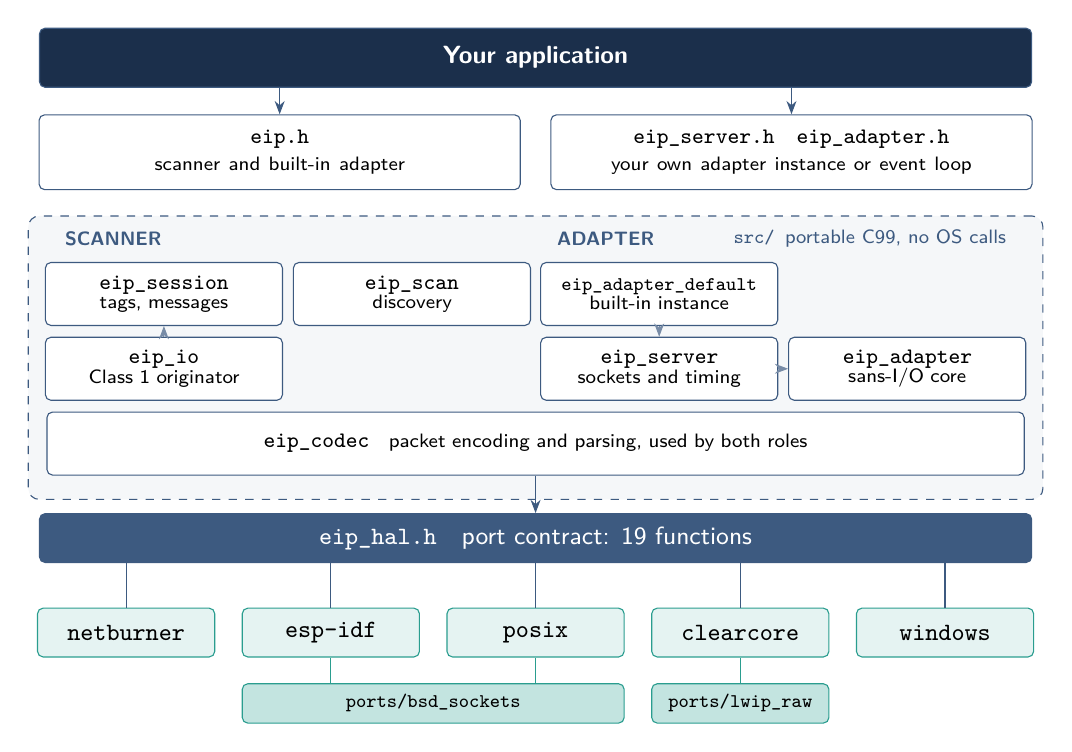
\begin{tikzpicture}[
  font=\sffamily\small,
  box/.style={draw=steel,fill=white,rounded corners=2pt,minimum height=0.62cm,inner sep=3pt,align=center},
  core/.style={box,fill=white,minimum width=2.95cm,text width=2.8cm,minimum height=0.8cm,font=\sffamily\scriptsize},
  port/.style={box,fill=teal!12,draw=teal,minimum width=2.25cm},
  shared/.style={box,fill=teal!28,draw=teal,minimum height=0.5cm,font=\sffamily\scriptsize},
  lbl/.style={font=\sffamily\scriptsize\bfseries\color{steel}}]

  % application
  \node[box,fill=navy,text=white,minimum width=12.6cm,minimum height=0.75cm] (app) at (0,6.75) {\bfseries Your application};

  % API headers
  \node[box,minimum width=6.1cm,text width=5.9cm,minimum height=0.95cm] (apiA) at (-3.25,5.55)
    {{\ttfamily\footnotesize eip.h}\\[-1pt]{\scriptsize scanner and built-in adapter}};
  \node[box,minimum width=6.1cm,text width=5.9cm,minimum height=0.95cm] (apiB) at ( 3.25,5.55)
    {{\ttfamily\footnotesize eip\_server.h\quad eip\_adapter.h}\\[-1pt]{\scriptsize your own adapter instance or event loop}};
  \draw[-Stealth,steel] (app.south -| apiA) -- (apiA);
  \draw[-Stealth,steel] (app.south -| apiB) -- (apiB);

  % core
  \node[lbl,anchor=west] at (-6.1,4.45) {SCANNER};
  \node[lbl,anchor=west] at ( 0.15,4.45) {ADAPTER};
  \node[font=\sffamily\scriptsize\color{steel},anchor=east] at (6.1,4.45) {\ttfamily src/\ \sffamily portable C99, no OS calls};
  \node[core] (s1) at (-4.72,3.75) {{\ttfamily\footnotesize eip\_session}\\[-1pt] tags, messages};
  \node[core] (s2) at (-4.72,2.80) {{\ttfamily\footnotesize eip\_io}\\[-1pt] Class 1 originator};
  \node[core] (s3) at (-1.57,3.75) {{\ttfamily\footnotesize eip\_scan}\\[-1pt] discovery};
  \node[core] (a1) at ( 1.57,3.75) {{\ttfamily\scriptsize eip\_adapter\_default}\\[-1pt] built-in instance};
  \node[core] (a2) at ( 1.57,2.80) {{\ttfamily\footnotesize eip\_server}\\[-1pt] sockets and timing};
  \node[core] (a3) at ( 4.72,2.80) {{\ttfamily\footnotesize eip\_adapter}\\[-1pt] sans-I/O core};
  \draw[-Stealth,steel!70] (a1) -- (a2);
  \draw[-Stealth,steel!70] (a2) -- (a3);
  \draw[-Stealth,steel!70] (s2) -- (s1);
  \node[core,minimum width=12.4cm,text width=12.2cm] (codec) at (0,1.85)
    {{\ttfamily\footnotesize eip\_codec}\quad packet encoding and parsing, used by both roles};
  \begin{scope}[on background layer]
    \node[draw=steel,dashed,rounded corners=4pt,fit=(s1)(s2)(s3)(a1)(a3)(codec),inner xsep=6pt,inner ysep=6pt,yshift=4pt,minimum height=3.6cm,fill=steel!5] (coreframe) {};
  \end{scope}

  % HAL bar
  \node[box,fill=steel,text=white,minimum width=12.6cm] (hal) at (0,0.65) {{\ttfamily eip\_hal.h}\quad port contract: 19 functions};
  \draw[-Stealth,steel] (codec.south) -- (hal.north);

  % ports
  \foreach \n/\x/\t in {pn/-5.2/netburner,pe/-2.6/esp-idf,pp/0/posix,pc/2.6/clearcore,pw/5.2/windows}{
    \node[port] (\n) at (\x,-0.55) {\ttfamily \t};
    \draw[steel] (hal.south -| \n) -- (\n.north);
  }
  \node[shared,minimum width=4.85cm] (bsd) at (-1.3,-1.45) {\ttfamily ports/bsd\_sockets};
  \node[shared,minimum width=2.25cm] (lw) at (2.6,-1.45) {\ttfamily ports/lwip\_raw};
  \draw[teal] (pe.south) -- (pe.south |- bsd.north);
  \draw[teal] (pp.south) -- (pp.south |- bsd.north);
  \draw[teal] (pc.south) -- (lw.north);
\end{tikzpicture}
\caption{The layers of QuickEIP. Arrows show the direction of calls. The
shared socket layers are reused by more than one platform port.}
\label{fig:layers}
\end{figure}

An application that has its own event loop can call the sans-I/O core in
\file{include/eip_adapter.h} directly. Most applications use \file{eip.h}
only.

\section{Source Files}\label{sec:sources}

Each build compiles three groups of files: the core, one port, and the
include paths. Table~\ref{tab:groups} lists them.

\begin{table}[htbp]
\centering
\caption{File groups in each build}\label{tab:groups}
\begin{tabularx}{\linewidth}{@{}P{0.16\linewidth}P{0.40\linewidth}L@{}}
\toprule
\textbf{Group} & \textbf{Files} & \textbf{Notes} \\
\midrule
Core & \file{src/eip_codec.c}, \file{src/eip_adapter.c},
\file{src/eip_session.c}, \file{src/eip_io.c}, \file{src/eip_scan.c},
\file{src/eip_server.c}, \file{src/eip_adapter_default.c}
& The same on all platforms. C99, no OS calls. \\
Port & One platform directory under \file{ports/}, plus a shared socket
layer for some platforms & Implements \file{include/eip_hal.h}. \\
Include paths & \file{include/} (public) and \file{src/} (internal headers
that the core needs) & Add both to the C and C++ compilers. \\
\bottomrule
\end{tabularx}
\end{table}

You can omit a core file if you do not use its functions.
Table~\ref{tab:corefiles} shows what each file is necessary for.

\begin{table}[htbp]
\centering
\caption{Core files and their functions}\label{tab:corefiles}
\begin{tabularx}{\linewidth}{@{}P{0.36\linewidth}L@{}}
\toprule
\textbf{File} & \textbf{Necessary for} \\
\midrule
\file{eip_codec.c} & All functions. \\
\file{eip_adapter.c}, \file{eip_server.c} & The adapter. \\
\file{eip_adapter_default.c} & \code{eip_adapter_start} and the other
built-in-instance calls. Holds a static \code{EipServer} of approximately
11~KB. \\
\file{eip_session.c} & Scanner sessions, tags, explicit messages, and
symbols. \\
\file{eip_io.c} & Scanner Class~1 I/O. Needs \file{eip_session.c}. \\
\file{eip_scan.c} & \code{eip_list_identity} and \code{eip_scan_devices}. \\
\bottomrule
\end{tabularx}
\end{table}

\begin{note}
\notelabel If you link with \code{-ffunction-sections -fdata-sections
-Wl,--gc-sections}, the linker removes the functions that you do not call.
Thus you can usually keep all the core files in the build.
\end{note}

\section{Execution Model}\label{sec:threads}

\subsection{The Adapter Context}

The adapter core runs in one context. On an RTOS port, this context is a task
that the port starts. On a bare-metal port, this context is your main loop,
which calls \code{eip_adapter_poll}. Table~\ref{tab:runmodes} compares the two
modes.

\begin{table}[htbp]
\centering
\caption{How the adapter runs}\label{tab:runmodes}
\begin{tabularx}{\linewidth}{@{}P{0.24\linewidth}P{0.26\linewidth}L@{}}
\toprule
\textbf{Mode} & \textbf{Ports} & \textbf{What you do} \\
\midrule
Task (RTOS) & NetBurner, ESP-IDF, POSIX, Windows & Nothing. \code{eip_adapter_start} starts a task. Do not call \code{eip_adapter_poll}. \\
Poll (bare metal) & ClearCore, other lwIP raw-API boards, Windows with \code{EIP_WIN_POLL_MODE} & Call \code{eip_adapter_poll} on each pass of the main loop, at intervals shorter than your fastest RPI. \\
\bottomrule
\end{tabularx}
\end{table}

\begin{caution}
Do not call \code{eip_adapter_poll} on an RTOS port. A task already runs the
adapter there. Two contexts that run the core at the same time can corrupt
the adapter state.
\end{caution}

\subsection{Rules for Tasks}

\begin{itemize}
  \item \code{eip_adapter_read}, \code{eip_adapter_write}, and
        \code{eip_adapter_snapshot} are safe from any task. They take
        \code{eip_hal_lock} for some microseconds. The lock is never held
        during a socket call.
  \item One task at a time can use a given \code{EipSession} or
        \code{EipIo}. Different sessions can run in different tasks.
  \item Scanner calls block until they are complete or until their timeout.
        On an RTOS, call them from a task of their own.
  \item On bare metal, a blocking scanner call keeps the network stack in
        operation, and the adapter sockets continue to receive packets. But
        the remainder of your main loop stops until the call returns.
  \item Do not call QuickEIP from an interrupt handler.
\end{itemize}

\section{Memory}\label{sec:memory}

QuickEIP uses no heap in the protocol code. Its RAM is static, or it is in
structures that you supply. Let $P$ be \code{EIP_MAX_PACKET} and let $C$ be
\code{EIP_ADAPTER_MAX_CLIENTS}. Then these approximations apply:
\begin{align}
  M_{\text{server}}  &\approx P\,(C + 3), \label{eq:server}\\
  M_{\text{session}} &\approx 3P. \label{eq:session}
\end{align}
With the defaults $P = 1536$ and $C = 4$, equation~\eqref{eq:server} gives
\num{10752} bytes, and equation~\eqref{eq:session} gives \num{4608} bytes plus
some fields. Table~\ref{tab:ram} gives the totals.

\begin{table}[htbp]
\centering
\caption{RAM with the default settings}\label{tab:ram}
\begin{tabularx}{\linewidth}{@{}P{0.38\linewidth}L@{}}
\toprule
\textbf{Item} & \textbf{RAM} \\
\midrule
Built-in adapter & Approximately 11~KB static, plus a 1.5~KB shared reply buffer. \\
Each \code{EipSession} & Approximately 4.7~KB. \\
Each \code{EipIo} & Approximately 100 bytes, plus a 1.5~KB stack buffer during produce and consume. \\
Scanner calls & Up to approximately 2~KB of caller stack. A tag write builds requests of 400 bytes. \\
Code, all functions & Approximately 24~KB at \code{-Os} on a Cortex-M4. \\
\bottomrule
\end{tabularx}
\end{table}

\begin{caution}
An \code{EipSession} is too large for most task stacks. Declare it
\code{static}, or put it in memory that you allocate one time at start-up.
A session on a small stack causes a stack overflow.
\end{caution}

The assembly data of the adapter comes from one pool. The sum of the sizes
$s_i$ of all assemblies must fit in it:
\begin{equation}
  \sum_{i=1}^{N} s_i \le \code{EIP_ADAPTER_DATA_POOL}, \qquad N \le \code{EIP_ADAPTER_MAX_ASSEMBLIES}.
  \label{eq:pool}
\end{equation}

\chapter{Building and Configuring QuickEIP}\label{ch:build}

\section{Build-Time Configuration}\label{sec:config}

All sizes are in \file{include/eip_config.h}. Each setting is a default in an
\code{\#ifndef} block. You can change a setting in two ways:

\begin{itemize}
  \item Give it with \code{-D} on the compiler command line.
  \item Put it in a header of your own, and compile with
        \code{-DEIP_CONFIG_FILE=\textbackslash"my_eip_config.h\textbackslash"}.
        \file{eip_config.h} includes that file first.
\end{itemize}

\begin{caution}
All files that include \file{eip.h} must see the same values, in C and in
C++. These settings change the size of structures. If two files see different
values, they disagree about the layout of \code{EipSession} or
\code{EipServer}, and memory becomes corrupt. Put the settings in a flag that
applies to the C and the C++ compiler, or use \code{EIP_CONFIG_FILE} for
both.
\end{caution}

\begin{procedure}{Change a build-time setting}
\begin{enumerate}
  \item Make a header, for example \file{my_eip_config.h}.
  \item Put one \code{\#define} in it for each setting that you change:
\begin{lstlisting}
/* my_eip_config.h */
#define EIP_ADAPTER_MAX_CLIENTS 2
#define EIP_ADAPTER_DATA_POOL   1024
\end{lstlisting}
  \item Add \code{-DEIP_CONFIG_FILE=\textbackslash"my_eip_config.h\textbackslash"}
        to the C compiler flags.
  \item Add the same flag to the C++ compiler flags.
  \item Do a clean build of all files.
\end{enumerate}
\end{procedure}

Table~\ref{tab:config} lists the settings.

\begin{table}[htbp]
\centering
\caption{Build-time settings in \file{eip_config.h}}\label{tab:config}
\small
\begin{tabularx}{\linewidth}{@{}P{0.36\linewidth}P{0.12\linewidth}L@{}}
\toprule
\textbf{Setting} & \textbf{Default} & \textbf{Effect} \\
\midrule
\code{EIP_MAX_PACKET} & 1536 & Largest encapsulation packet. The minimum is 1024, and a smaller value stops the build. It sizes the session buffers (3$\times$), the server reply buffers (2$\times$), and each adapter TCP client (1$\times$). \\
\code{EIP_ADAPTER_MAX_ASSEMBLIES} & 8 & Assembly instances in each adapter. \\
\code{EIP_ADAPTER_DATA_POOL} & 512 & Bytes that all assembly data shares. \\
\code{EIP_ADAPTER_MAX_CLIENTS} & 4 & Explicit-message (TCP) sessions at the same time. Each costs approximately \code{EIP_MAX_PACKET} bytes. \\
\code{EIP_ADAPTER_EVICT_MS} & 60000 & If all TCP slots are busy, the adapter drops a session that has been silent this long, for a new client. It never drops the session of the Class~1 owner. \\
\code{EIP_ADAPTER_UDP_REPLY_MS} & 20 & Interval at which the UDP 44818 rate limit adds one token. \\
\code{EIP_ADAPTER_UDP_REPLY_BURST} & 20 & Maximum number of stored tokens. \\
\code{EIP_ADAPTER_IDLE_WAIT_MS} & 5 & Longest wait in one call to \code{eip_server_service}. \\
\code{EIP_ADAPTER_TASK_STACK} & 0 & Adapter task stack, in the units of the RTOS. 0 selects the port default. \\
\code{EIP_ADAPTER_TASK_PRIORITY} & 0 & Adapter task priority, in the units of the RTOS. 0 selects the port default. \\
\bottomrule
\end{tabularx}
\end{table}

\subsection{The UDP Reply Rate Limit}

The adapter answers ListIdentity and ListServices on UDP 44818 through a
token bucket. Each reply uses one token. Let $R$ be
\code{EIP_ADAPTER_UDP_REPLY_MS} and let $B$ be
\code{EIP_ADAPTER_UDP_REPLY_BURST}. Then, in a time $t$, the adapter sends no
more than this number of replies:
\begin{equation}
  n_{\max}(t) = B + \left\lfloor \frac{t}{R} \right\rfloor.
\end{equation}
With the defaults, the adapter answers a burst of 20 requests and then 50
requests per second. A broadcast storm thus cannot stop Class~1 I/O. The
snapshot field \code{udp_replies_dropped} counts the requests that the
adapter did not answer.

\subsection{Task Settings}

The two task settings have a meaning on some ports only.
Table~\ref{tab:tasksettings} shows which.

\begin{table}[htbp]
\centering
\caption{Use of the task settings by port}\label{tab:tasksettings}
\begin{tabularx}{\linewidth}{@{}P{0.22\linewidth}P{0.30\linewidth}L@{}}
\toprule
\textbf{Port} & \textbf{\code{EIP_ADAPTER_TASK_STACK}} & \textbf{\code{EIP_ADAPTER_TASK_PRIORITY}} \\
\midrule
ESP-IDF & Bytes (default 6144) & FreeRTOS priority (default 12) \\
NetBurner & Not used (NNDK default stack) & NBRTOS priority (default \code{MAIN_PRIO - 1}) \\
Windows & Bytes (0: system default) & A \code{THREAD_PRIORITY_*} value (0: \code{THREAD_PRIORITY_HIGHEST}) \\
POSIX & Not used & Not used \\
ClearCore & Not used (no task) & Not used (no task) \\
\bottomrule
\end{tabularx}
\end{table}

\section{Host Build}\label{sec:hostbuild}

The host build uses CMake. It needs CMake 3.13 or later and a C99 compiler. It
operates on Linux, macOS, WSL, and Windows with Visual Studio.

\begin{procedure}{Build and test on Linux, macOS, or WSL}
\begin{enumerate}
  \item Go to the root of the repository.
  \item Configure the build:
\begin{lstlisting}[language=shell]
cmake -S . -B build
\end{lstlisting}
  \item Compile:
\begin{lstlisting}[language=shell]
cmake --build build
\end{lstlisting}
  \item Run the tests:
\begin{lstlisting}[language=shell]
ctest --test-dir build --output-on-failure
\end{lstlisting}
  \item Make sure that all tests pass.
\end{enumerate}
\end{procedure}

\begin{procedure}{Build and test on Windows with Visual Studio}
\begin{enumerate}
  \item Open a Developer Command Prompt at the root of the repository.
  \item Configure the build:
\begin{lstlisting}[language=shell]
cmake -S . -B build
\end{lstlisting}
  \item Compile the Release configuration:
\begin{lstlisting}[language=shell]
cmake --build build --config Release
\end{lstlisting}
  \item Run the tests:
\begin{lstlisting}[language=shell]
ctest --test-dir build -C Release --output-on-failure
\end{lstlisting}
  \item Make sure that all tests pass.
\end{enumerate}
\end{procedure}

\subsection{Targets and Options}

Table~\ref{tab:targets} lists the CMake targets. Two options control the
optional targets: \code{QUICKEIP_BUILD_TESTS} and \code{QUICKEIP_BUILD_TOOLS}.
Both are \code{ON} by default.

\begin{table}[htbp]
\centering
\caption{CMake targets}\label{tab:targets}
\begin{tabularx}{\linewidth}{@{}P{0.32\linewidth}L@{}}
\toprule
\textbf{Target} & \textbf{Contents} \\
\midrule
\code{quickeip_core} & The portable core only. Link your own \code{eip_hal_*} port. \\
\code{quickeip} & The core plus the host port (POSIX or Windows). \\
\code{eiptool} & The command-line tool. Set \code{-DQUICKEIP_BUILD_TOOLS=OFF} to omit it. \\
\code{test_core}, \code{test_session}, \code{test_hal}, \code{test_loopback} & The tests. Set \code{-DQUICKEIP_BUILD_TESTS=OFF} to omit them. \\
\bottomrule
\end{tabularx}
\end{table}

\subsection{Tests}\label{sec:tests}

Table~\ref{tab:tests} describes each test and what it needs.

\begin{table}[htbp]
\centering
\caption{Tests}\label{tab:tests}
\small
\begin{tabularx}{\linewidth}{@{}P{0.16\linewidth}LP{0.25\linewidth}@{}}
\toprule
\textbf{Test} & \textbf{Covers} & \textbf{Needs} \\
\midrule
\code{test_core} & The codec and the adapter core, byte for byte. Includes Forward\_Open captures from real devices. & Nothing: no sockets and no clock. \\
\code{test_session} & The scanner session against a scripted device, through a fake HAL. Routed requests, router failures, and late, short, and too-large replies. & Nothing: no sockets and no clock. \\
\code{test_hal} & The port contract, through the loopback interface of the host. Busy ports fail, long datagrams are cut, ICMP errors are not fatal, timeouts hold, and the clock steps at its stated resolution. & Free TCP and UDP ports in the 478xx range. \\
\code{test_loopback} & The scanner against the adapter through the host port. Discovery, explicit messages, Class~1 in the two directions, idle, the watchdog, and reopen. & A non-loopback interface. TCP and UDP 44818 and UDP 2222 must be free. \\
\bottomrule
\end{tabularx}
\end{table}

\begin{note}
\notelabel If another EtherNet/IP program on the host uses port 44818 or 2222,
\code{test_loopback} fails. Stop that program, and then run the test again.
\end{note}

\section{Use QuickEIP in Your Own CMake Project}\label{sec:owncmake}

\begin{procedure}{Add QuickEIP to a CMake project}
\begin{enumerate}
  \item Put the QuickEIP repository beside your project, or in a
        subdirectory of it.
  \item Set the two build options to \code{OFF} before
        \code{add_subdirectory}. If you do not, the tests and
        \code{eiptool} also compile.
  \item Add QuickEIP with \code{add_subdirectory}.
  \item Link your target to \code{quickeip}. This gives the include paths
        and the thread library.
\end{enumerate}
\end{procedure}

\begin{lstlisting}[language=cmake]
cmake_minimum_required(VERSION 3.13)
project(myapp C)

set(QUICKEIP_BUILD_TESTS OFF CACHE BOOL "")
set(QUICKEIP_BUILD_TOOLS OFF CACHE BOOL "")
add_subdirectory(../QuickEIP quickeip)

add_executable(myapp main.c)
target_link_libraries(myapp PRIVATE quickeip)
\end{lstlisting}

For an embedded target without CMake, compile the core files of
table~\ref{tab:groups} and one port, and add \file{include/} and \file{src/}
to the include paths. Chapter~\ref{ch:platforms} gives the steps for each
shipped platform.

\chapter{Implementing an Adapter}\label{ch:adapter}

An adapter makes your device an EtherNet/IP I/O device. A PLC opens a Class~1
connection to it and exchanges assembly data at a fixed interval, the RPI.
This chapter tells you how to start the adapter, exchange data, and set the
assemblies so that a PLC accepts them.

\section{Assemblies}\label{sec:assemblies}

An \term{assembly} is a block of bytes with an instance number. The adapter
has three types of assembly. Table~\ref{tab:asmtypes} gives their directions.

\begin{table}[htbp]
\centering
\caption{Assembly types}\label{tab:asmtypes}
\begin{tabularx}{\linewidth}{@{}P{0.25\linewidth}P{0.14\linewidth}L@{}}
\toprule
\textbf{Type} & \textbf{Direction} & \textbf{Meaning} \\
\midrule
\code{EIP_ASM_CONSUMED} & \OT & Data that the PLC writes. Your application reads it. \\
\code{EIP_ASM_PRODUCED} & \TO & Data that your application writes. The PLC reads it. \\
\code{EIP_ASM_CONFIG} & In the Forward\_Open & Configuration data. Size 0 is permitted. \\
\bottomrule
\end{tabularx}
\end{table}

\begin{caution}
Do not mix up the two directions. Consumed is what the PLC writes, and
produced is what the PLC reads. The built-in test set uses instance 100 as
consumed. The examples in this manual use instance 100 as produced.
\end{caution}

You select the instance numbers. This manual uses 150 (consumed, 32 bytes),
100 (produced, 32 bytes), and 151 (config, 0 bytes). If you give no
configuration, the adapter uses a built-in test set (table~\ref{tab:testset}).

\begin{table}[htbp]
\centering
\caption{The built-in test set (\code{config} or \code{assembly_count} is 0)}\label{tab:testset}
\begin{tabularx}{\linewidth}{@{}P{0.14\linewidth}P{0.20\linewidth}P{0.12\linewidth}L@{}}
\toprule
\textbf{Instance} & \textbf{Direction} & \textbf{Bytes} & \textbf{Notes} \\
\midrule
100 & Consumed & 8 & \\
101 & Produced & 8 & Initial data \code{11 22 33 44 55 66 77 88}. \\
102 & Produced & 4 & \\
150 & Config & 4 & \\
\bottomrule
\end{tabularx}
\end{table}

With \code{vendor_id} 0, the adapter also uses a test identity: vendor 65000
and product name ``EIP Test Adapter.''

\section{Start the Adapter}\label{sec:start}

\begin{procedure}{Start the built-in adapter}
\begin{enumerate}
  \item Declare an array of \code{EipAssemblyConfig}, one entry for each
        assembly.
  \item Declare an \code{EipAdapterConfig} and set all of it to zero with
        \code{memset}.
  \item Set the identity fields: \code{vendor_id}, \code{device_type},
        \code{product_code}, \code{revision_major}, \code{revision_minor}, and
        \code{product_name}.
  \item Set \code{assemblies} and \code{assembly_count}.
  \item Set the optional fields and callbacks (section~\ref{sec:callbacks}).
  \item Call \code{eip_adapter_start}.
  \item Make sure that the return value is \code{EIP_OK}.
  \item On a poll-mode port only, call \code{eip_adapter_poll} on each pass
        of the main loop.
\end{enumerate}
\end{procedure}

\begin{lstlisting}
#include <string.h>
#include "eip.h"

static const EipAssemblyConfig kAssemblies[] = {
    /* instance, direction,   size, name,     initial, implicit_only */
    {150, EIP_ASM_CONSUMED, 32, "Outputs", 0, 0},   /* O->T: the PLC writes it  */
    {100, EIP_ASM_PRODUCED, 32, "Inputs",  0, 0},   /* T->O: we send it         */
    {151, EIP_ASM_CONFIG,    0, "Config",  0, 0},   /* config point of the path */
};

int start_eip(void)
{
    EipAdapterConfig cfg;

    memset(&cfg, 0, sizeof cfg);
    cfg.vendor_id = 65000;            /* placeholder: use your ODVA vendor id */
    cfg.device_type = 43;             /* 43 generic device, 12 comms adapter */
    cfg.product_code = 1;
    cfg.revision_major = 1;
    cfg.revision_minor = 1;           /* an EDS needs 1 or higher */
    cfg.product_name = "My Device";   /* up to 31 characters */
    cfg.serial_number = 0;            /* 0: derived from the MAC */
    cfg.assemblies = kAssemblies;
    cfg.assembly_count = 3;
    return eip_adapter_start(&cfg);   /* copies what it needs from cfg */
}
\end{lstlisting}

\begin{caution}
Set all fields of \code{EipAdapterConfig}, including \code{link_info} and the
other callbacks, before you call \code{eip_adapter_start}. The function copies
the configuration. A change after the call has no effect.
\end{caution}

\begin{note}
\notelabel Vendor ID 65000 is a placeholder. Get your own vendor ID from
ODVA, and use it in the device and in its EDS file.
\end{note}

\code{eip_adapter_start} copies what it needs, so \code{cfg} and the assembly
array can be on the stack. The adapter listens on TCP 44818, UDP 44818, and
UDP 2222. If the network is not ready, the adapter tries again to open its
sockets one time each second. The field \code{listening} in
\code{EipAdapterView} becomes 1 when the sockets are open.

\section{Exchange Data}\label{sec:exchange}

Use \code{eip_adapter_read} to get the data that the PLC sent. Use
\code{eip_adapter_write} to set the data that the PLC receives.

\begin{lstlisting}
uint8_t out[32], in[32];
uint16_t len = sizeof out;

eip_adapter_read(150, out, &len);   /* latest data from the PLC          */
/* ... use out, fill in ... */
eip_adapter_write(100, in, 32);     /* sent on the next T->O packet      */
\end{lstlisting}

These rules apply:

\begin{itemize}
  \item The two calls are safe from any task.
  \item \code{eip_adapter_write} needs the exact size of the assembly.
  \item For \code{eip_adapter_read}, \code{data_len} is the capacity on input
        and the byte count on output. A capacity smaller than the assembly is
        \code{EIP_ERR_TOO_BIG}.
  \item An unknown instance returns \code{EIP_ERR_PATH}.
\end{itemize}

\subsection{The Safe State of Consumed Data}\label{sec:safestate}

The consumed assembly reads as all zeros in these conditions:

\begin{itemize}
  \item The connection timed out or closed.
  \item The PLC is in Program mode. The run/idle header then says ``idle.''
\end{itemize}

Before the first connection, the consumed assembly reads as its
\code{initial} data. That data is also zeros if you do not set it.
Figure~\ref{fig:safestate} shows the states.

\begin{figure}[htbp]
\centering
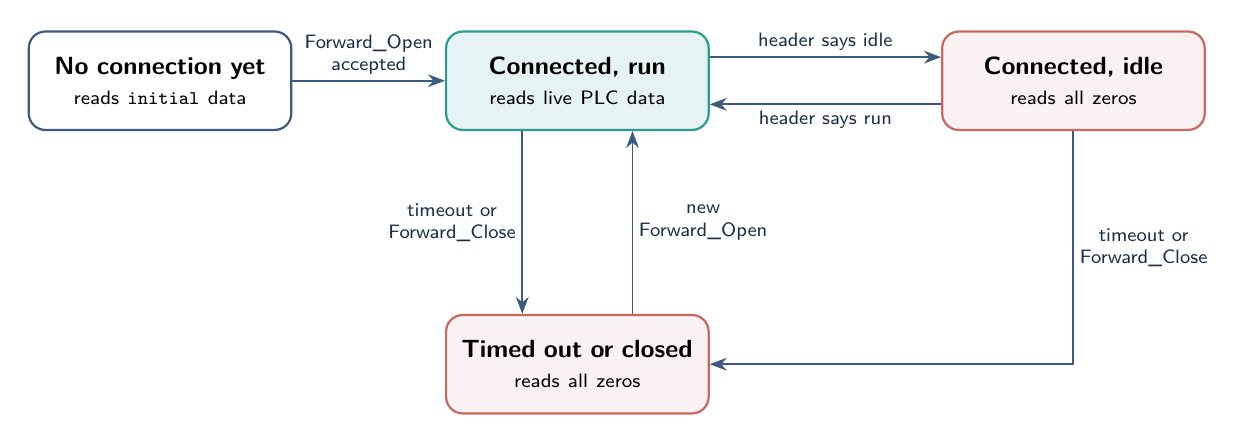
\begin{tikzpicture}[
  font=\sffamily\small,>=Stealth,
  st/.style={draw=steel,fill=white,rounded corners=6pt,minimum width=3.3cm,text width=3.1cm,minimum height=1.25cm,align=center,line width=0.8pt},
  zero/.style={st,fill=signal!6,draw=signal!70},
  live/.style={st,fill=teal!12,draw=teal},
  tr/.style={->,steel,line width=0.7pt},
  lab/.style={font=\sffamily\scriptsize,inner sep=2pt,align=center,text=navy}]
  \node[st] (init) at (0,0) {\textbf{No connection yet}\\\scriptsize reads \code{initial} data};
  \node[live] (run) at (5.3,0) {\textbf{Connected, run}\\\scriptsize reads live PLC data};
  \node[zero] (idle) at (11.6,0) {\textbf{Connected, idle}\\\scriptsize reads all zeros};
  \node[zero] (closed) at (5.3,-3.6) {\textbf{Timed out or closed}\\\scriptsize reads all zeros};
  \draw[tr] (init) -- node[lab,above]{Forward\_Open\\accepted} (run);
  \draw[tr] ([yshift=3mm]run.east) -- node[lab,above]{header says idle} ([yshift=3mm]idle.west);
  \draw[tr] ([yshift=-3mm]idle.west) -- node[lab,below]{header says run} ([yshift=-3mm]run.east);
  \draw[tr] ([xshift=-7mm]run.south) -- node[lab,left]{timeout or\\Forward\_Close} ([xshift=-7mm]closed.north);
  \draw[tr] ([xshift=7mm]closed.north) -- node[lab,right]{new\\Forward\_Open} ([xshift=7mm]run.south);
  \draw[tr] (idle.south) |- node[lab,pos=0.25,right]{timeout or\\Forward\_Close} (closed.east);
\end{tikzpicture}
\caption{States of the consumed assembly. Red states read as all zeros. A
modeless connection, which has no run/idle header, stays in ``run.''}
\label{fig:safestate}
\end{figure}

\begin{warning}
Design your application so that all-zero consumed data puts your machine
in a safe condition. When the connection stops, or when the PLC goes to
Program mode, your outputs see zeros. If zero is not a safe value for an
output, add logic that makes it safe. Do not use this function as a safety
function.
\end{warning}

\subsection{Status and Diagnostics}

\code{eip_adapter_snapshot} copies the adapter state into an
\code{EipAdapterView}. It gives the identity, the connection state, the RPI,
the inactivity timeout, and these counters:

\begin{itemize}
  \item packets in and out, and successful opens and timeouts
  \item drops by cause: old sequence number (\code{rx_dropped_seq}), wrong
        source address (\code{rx_dropped_source}), and malformed packet
        (\code{rx_dropped_bad})
  \item packets accepted in idle (\code{rx_idle}), and UDP replies not sent
        (\code{udp_replies_dropped})
\end{itemize}

Use these values on a status page. Appendix~\ref{app:types} lists all
fields. The Identity object status word also shows the state:
\hex{0034} with no connection, \hex{0065} in run, and \hex{0075} in idle.

\section{Assemblies, Sizes, and the EDS File}\label{sec:sizes}

The PLC sets up the connection from your EDS file. The adapter refuses a
Forward\_Open that does not agree with its assemblies.

\subsection{Assembly Size and Wire Size}

In an EDS file and in PLC software, you enter the \emph{assembly} size. The
2-byte sequence count and the 4-byte run/idle header are added on the wire.
The adapter checks the wire size. Let $n$ be the assembly size in bytes, and
let $h$ be 1 if the direction has a run/idle header, else 0. Then:
\begin{align}
  S_{\OT} &= 2 + 4h + n, \label{eq:o2t}\\
  S_{\TO} &= 2 + n. \label{eq:t2o}
\end{align}
For a 32-byte assembly in each direction, $S_{\OT} = 38$ and $S_{\TO} = 34$.
Figure~\ref{fig:o2t} shows where these bytes are in an \OT{} packet.

\begin{figure}[htbp]
\centering
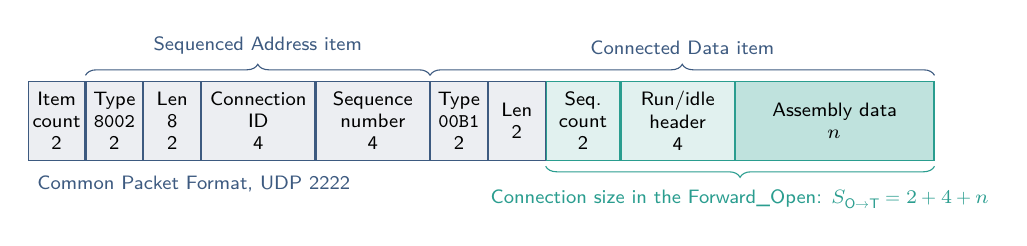
\begin{tikzpicture}[font=\sffamily\scriptsize,
  f/.style={draw=steel,minimum height=1.0cm,align=center,inner sep=1pt,fill=white},
  g/.style={f,fill=steel!10},
  c/.style={f,fill=teal!14,draw=teal},
  d/.style={f,fill=teal!30,draw=teal}]
  \def\u{0.36}
  \node[g,minimum width=2*\u cm] (a) at (0,0) {Item\\count\\2};
  \node[g,minimum width=2*\u cm,right=0pt of a] (b) {Type\\\texttt{8002}\\2};
  \node[g,minimum width=2*\u cm,right=0pt of b] (c) {Len\\8\\2};
  \node[g,minimum width=4*\u cm,right=0pt of c] (e) {Connection\\ID\\4};
  \node[g,minimum width=4*\u cm,right=0pt of e] (h) {Sequence\\number\\4};
  \node[g,minimum width=2*\u cm,right=0pt of h] (i) {Type\\\texttt{00B1}\\2};
  \node[g,minimum width=2*\u cm,right=0pt of i] (j) {Len\\2};
  \node[c,minimum width=2.6*\u cm,right=0pt of j] (k) {Seq.\\count\\2};
  \node[c,minimum width=4*\u cm,right=0pt of k] (l) {Run/idle\\header\\4};
  \node[d,minimum width=7*\u cm,right=0pt of l] (m) {Assembly data\\$n$};
  \draw[decorate,decoration={brace,amplitude=4pt},steel] ([yshift=2pt]b.north west) -- node[above=4pt,align=center]{Sequenced Address item} ([yshift=2pt]h.north east);
  \draw[decorate,decoration={brace,amplitude=4pt},steel] ([yshift=2pt]i.north west) -- node[above=4pt,align=center]{Connected Data item} ([yshift=2pt]m.north east);
  \draw[decorate,decoration={brace,amplitude=4pt,mirror},teal] ([yshift=-2pt]k.south west) -- node[below=5pt,align=center]{Connection size in the Forward\_Open: $S_{\OT} = 2 + 4 + n$} ([yshift=-2pt]m.south east);
  \node[anchor=north west,text=steel] at ([yshift=-2pt]a.south west) {Common Packet Format, UDP 2222};
\end{tikzpicture}
\caption{An \OT{} Class~1 packet with a run/idle header. Sizes are in bytes.
A \TO{} packet has the same items but normally no run/idle header.}
\label{fig:o2t}
\end{figure}

The run/idle header is a format flag in the EDS file. It is not part of the
size that you enter.

\subsection{Rules for a Forward\_Open}\label{sec:forwardopen}

Table~\ref{tab:forwardopen} gives the rules that the adapter applies to a
Forward\_Open, and the status that it returns when a rule is not met. The
sizes in this table are wire sizes.

\begin{table}[htbp]
\centering
\caption{Forward\_Open rules and the error status for each}\label{tab:forwardopen}
\small
\begin{tabularx}{\linewidth}{@{}LP{0.30\linewidth}@{}}
\toprule
\textbf{Rule} & \textbf{Status if not met} \\
\midrule
The connection path names an existing consumed, produced, and config instance. & \hex{01} / \hex{012A} (consumed), \hex{012B} (produced), \hex{0129} (config) \\
\OT{} size $= 2 + 4h + n$ (equation~\ref{eq:o2t}). & \hex{01} / \hex{0127} \\
\TO{} size $= 2 + n$. If the size also includes a 4-byte header, the adapter accepts it and sends a header that always says ``run.'' & \hex{01} / \hex{0128} \\
Config data in the path, if any, is equal to the config assembly size. & \hex{01} / \hex{0126} \\
The electronic key, if the PLC checks it, agrees with the vendor, device type, product code, and revision. A zero in the key agrees with all values. & \hex{01} / \hex{0114}--\hex{0116} \\
No other originator owns the connection. & \hex{01} / \hex{0106}, or \hex{01} / \hex{0113} if the request has no \OT \\
\bottomrule
\end{tabularx}
\end{table}

A size-0 \code{EIP_ASM_CONFIG} assembly accepts a path with a config point
and no data. Most PLCs send that. Set \code{implicit_only} to 1 to hide an
assembly from explicit Get and Set (status \hex{16}). Class~1 can still use
that assembly.

\subsection{The Inactivity Timeout}\label{sec:timeout}

The adapter closes the connection if no valid \OT{} packet arrives in the
inactivity timeout. The timeout comes from the \OT{} RPI and the timeout
multiplier $m$ (0--7) in the Forward\_Open.\footnote{ODVA, \textit{The CIP
Networks Library}, vol.~1, \textit{Common Industrial Protocol}, chap.~3,
Connection Manager object.} Let $T_{\text{f}}$ be
\code{timeout_floor_ms} and let $\Delta$ be the clock resolution of the port:
\begin{equation}
  T_{\text{inactivity}} = \max\!\left(\text{RPI}_{\OT} \cdot 4 \cdot 2^{m},\;
  T_{\text{f}},\; 2\Delta\right).
  \label{eq:timeout}
\end{equation}
The result is rounded up to whole ticks. In ticks, it is also limited to
\hex{00FFFFFF}. For example, a Micro850 sends an RPI of 50~ms with $m = 0$,
so $T_{\text{inactivity}} = 50 \times 4 = 200$~ms. A multiplier of 2 with a
10~ms RPI gives $10 \times 16 = 160$~ms.

\begin{note}
\notelabel On a platform that is not real time, such as Windows, set
\code{timeout_floor_ms} to 500 or more. A 100~ms stall of the host then does
not close the connection.
\end{note}

\subsection{Multicast \TO}

If the PLC requests a multicast \TO{} connection, the adapter selects the
group address from its own IP address $a$ and its network mask $k$, as the
EtherNet/IP specification tells.\footnote{ODVA, \textit{The CIP Networks
Library}, vol.~2, \textit{EtherNet/IP Adaptation of CIP}, sec.~3-5.3.} Let the
host ID be $h = a \wedge \lnot k$. Then:
\begin{equation}
  A_{\text{mcast}} = 239.192.1.0 + 32 \cdot \bigl((h - 1) \wedge \hex{3FF}\bigr).
\end{equation}
Multicast does not let a second originator listen. The adapter still accepts
one Class~1 connection only.

\section{Optional Callbacks}\label{sec:callbacks}

Table~\ref{tab:callbacks} lists the callbacks in \code{EipAdapterConfig}. All
of them run in the adapter context, the task or \code{eip_adapter_poll}. Each
receives \code{callback_ctx} as its first argument.

\begin{table}[htbp]
\centering
\caption{Adapter callbacks}\label{tab:callbacks}
\small
\begin{tabularx}{\linewidth}{@{}P{0.17\linewidth}P{0.27\linewidth}L@{}}
\toprule
\textbf{Field} & \textbf{When it is called} & \textbf{Use} \\
\midrule
\code{link_info} & Each 100 ms & Gives link state, speed, and duplex for the Ethernet Link object, if the port cannot read them (ESP-IDF). Return 1 while the link is up, and 0 to report it down. \\
\code{apply_interface} & Approximately 150 ms after a scanner sets TCP/IP Interface attribute 3, 5, or 6. The reply has already gone out. & Store and apply the new IP settings. Set it to 0 to make those attributes read-only. \\
\code{reset} & Approximately 300 ms after an Identity Reset request & Restart (type 0), or set the factory settings and restart (type 1). Set it to 0 to refuse the service. \\
\code{allow_change} & Before the adapter accepts a TCP/IP Interface Set or an Identity Reset & Return 0 to permit the change. Return a CIP general status, usually \hex{10} (device state conflict), to refuse it. \\
\bottomrule
\end{tabularx}
\end{table}

\begin{warning}
A scanner on the network can send an Identity Reset or change the IP address
of your device. If your device controls machinery, supply
\code{allow_change}. Make it refuse these requests while the machinery can
move.
\end{warning}

\begin{caution}
\code{allow_change} runs while the adapter holds \code{eip_hal_lock}. Keep it
short. Do not call an \code{eip_adapter_*} function from it, because that
function also takes the lock.
\end{caution}

A request that \code{allow_change} refuses never gets to
\code{apply_interface} or \code{reset}.

\section{More Control: The EipServer API}\label{sec:eipserver}

The functions \code{eip_adapter_*} use one built-in instance of
\code{EipServer}. The header \file{eip_server.h} gives access to that type.
Use it for these tasks:

\begin{itemize}
  \item Put the 11~KB server in memory that you select.
  \item Run the loop from your own task.
  \item Stop the adapter and start it again.
\end{itemize}

\begin{lstlisting}
static EipServer server;

eip_server_init(&server, &config);
for (;;) {
    eip_server_service(&server, 5);   /* RTOS task: waits up to 5 ms */
}
/* bare metal: call eip_server_poll(&server) from the main loop instead */
\end{lstlisting}

\code{eip_server_init}, \code{eip_server_poll}, \code{eip_server_service},
and \code{eip_server_close} run in one context. \code{eip_server_read},
\code{eip_server_write}, and \code{eip_server_snapshot} are safe from any
task, because they take \code{eip_hal_lock}.

\subsection{The Sans-I/O Core}

The header \file{eip_adapter.h} gives the core under the server. The core
never uses a socket or a clock. You give it packets and a tick count, and you
send the packets that it returns. Use it only if you write your own event
loop. The core has one shared reply buffer. Thus you must serialize the calls
on all \code{EipAdapter} objects in a program. Appendix~\ref{app:api} lists
its functions.

\chapter{Connecting a PLC to the Adapter}\label{ch:plc}

This chapter tells you how to make an EDS file for your adapter and how to
connect a PLC to it. Do the checks in section~\ref{sec:precheck} before you
start the PLC software.

\section{Checks Before You Use the PLC}\label{sec:precheck}

\begin{procedure}{Check the adapter from a PC}
\begin{enumerate}
  \item Connect a PC to the same network as the adapter.
  \item Build \code{eiptool} on the PC (section~\ref{sec:hostbuild}).
  \item Read the identity of the adapter:
\begin{lstlisting}[language=shell]
eiptool identity <adapter-ip>
\end{lstlisting}
  \item Make sure that the vendor, product code, and name are correct.
  \item Read the data of the produced assembly:
\begin{lstlisting}[language=shell]
eiptool get <adapter-ip> 4 100 3
\end{lstlisting}
  \item Make sure that the byte count is equal to the assembly size.
\end{enumerate}
\end{procedure}

\section{Make the EDS File}\label{sec:eds}

The file \file{examples/eds/QuickEIP_Adapter.eds} agrees with the assemblies
in section~\ref{sec:start}. Use it as the start for your EDS file.
Table~\ref{tab:edsfields} shows which values must agree with your
configuration.

\begin{table}[htbp]
\centering
\caption{EDS fields and the configuration values that they must agree with}\label{tab:edsfields}
\small
\begin{tabularx}{\linewidth}{@{}P{0.38\linewidth}L@{}}
\toprule
\textbf{EDS field} & \textbf{Must be equal to} \\
\midrule
\code{VendCode}, \code{ProdType}, \code{ProdCode} & \code{vendor_id}, \code{device_type}, \code{product_code} \\
\code{MajRev}, \code{MinRev} & \code{revision_major}, \code{revision_minor}. EDS tools need 1--255, so do not use a minor revision of 0. \\
\code{ProdName} & \code{product_name} \\
\code{VendName}, \code{Catalog} & Your company and your part number. No configuration field agrees with these. \\
\code{Assem}\textit{NNN}, its size, and its member size in bits & An \code{EipAssemblyConfig} instance, its \code{size}, and \code{size} $\times$ 8 \\
Connection sizes, \code{TSpec1}, \code{TSpec2} & The assembly sizes (not the wire sizes) \\
\code{Number_Of_Static_Instances} under \code{[Assembly]} & \code{assembly_count} \\
Connection path & \code{20 04 24} \textit{config} \code{2C} \textit{consumed} \code{2C} \textit{produced}, with instances in hexadecimal, for instances up to 255 \\
Assembly path & \code{20 04 24} \textit{instance} \code{30 03}, with the instance in hexadecimal \\
\bottomrule
\end{tabularx}
\end{table}

For the example assemblies, config 151 is \hex{97}, consumed 150 is \hex{96},
and produced 100 is \hex{64}. Thus the connection path is
\code{20 04 24 97 2C 96 2C 64}.

\begin{procedure}{Adapt the sample EDS file}
\begin{enumerate}
  \item Copy \file{examples/eds/QuickEIP_Adapter.eds} and give the copy a new name.
  \item Set the \code{[Device]} values from table~\ref{tab:edsfields}.
  \item Set each \code{Assem}\textit{NNN} entry to agree with one assembly.
  \item Set the connection sizes and \code{TSpec1} and \code{TSpec2} to the assembly sizes.
  \item Set the connection path to your config, consumed, and produced instances.
  \item Do not change the other values.
  \item Do the checks of section~\ref{sec:precheck} again.
\end{enumerate}
\end{procedure}

\begin{caution}
When an assembly layout changes, also change \code{ProdCode} or the revision.
If you do not, a PLC can use an old EDS file with the new device, and the
data has a different meaning.
\end{caution}

\begin{note}
\notelabel The connection values in the sample file were checked: they opened
a connection to a running adapter. But nobody has imported the file itself
into PLC software yet.
\end{note}

Appendix~\ref{app:tools} contains the important parts of the sample file.

\section{Micro850 (Connected Components Workbench)}

This setup was tested with the ClearCore port.

\begin{procedure}{Connect a Micro850}
\begin{enumerate}
  \item In Connected Components Workbench, add a generic EtherNet/IP device.
  \item Set its address to the address of the adapter.
  \item Set the output assembly (\OT) to instance 150, 32 bytes.
  \item Set the input assembly (\TO) to instance 100, 32 bytes.
  \item Set the config assembly to instance 151, 0 bytes.
  \item Download the project to the controller.
  \item Put the controller in Run mode.
  \item On the adapter, make sure that \code{io_open} and \code{run} are 1 in
        the snapshot.
\end{enumerate}
\end{procedure}

Table~\ref{tab:micro850} shows the values that a Micro850 was seen to send.

\begin{table}[htbp]
\centering
\caption{Connection values sent by a Micro850}\label{tab:micro850}
\begin{tabularx}{\linewidth}{@{}P{0.32\linewidth}L@{}}
\toprule
\textbf{Setting} & \textbf{Value} \\
\midrule
RPI & 50 ms in each direction \\
\OT & Point-to-point, with the run/idle header \\
\TO & No header \\
Timeout multiplier & 0 ($\times$4, thus 200 ms at a 50 ms RPI) \\
Electronic key & All zeros \\
Config & Names the config instance and sends no data \\
\bottomrule
\end{tabularx}
\end{table}

The config instance must exist. If it does not, the adapter refuses the open
with \hex{01} / \hex{0129}. A size-0 \code{EIP_ASM_CONFIG} assembly is
sufficient.

\section{CompactLogix and ControlLogix (Studio 5000)}

This adapter has not been tested with these controllers. But an EDS file with
the same connection values, and generic module settings in this form, have
operated on a CompactLogix with a different adapter.

You can install the EDS file with the \menu{EDS Hardware Installation Tool}
and add the device as a module. Or you can add a \menu{Generic Ethernet
Module} with the values in table~\ref{tab:generic}.

\begin{table}[htbp]
\centering
\caption{Generic Ethernet Module settings}\label{tab:generic}
\begin{tabularx}{\linewidth}{@{}P{0.32\linewidth}L@{}}
\toprule
\textbf{Field} & \textbf{Value} \\
\midrule
\menu{Comm Format} & Data -- SINT \\
\menu{IP Address} & The address of the adapter \\
\menu{Input} & Assembly instance 100, size 32 \\
\menu{Output} & Assembly instance 150, size 32 \\
\menu{Configuration} & Assembly instance 151, size 0 \\
\bottomrule
\end{tabularx}
\end{table}

Then set the RPI on the \menu{Connection} tab. In the two methods, the config
assembly must exist on the adapter, also at size 0. It comes first in the
connection path.

\section{Adapter on a PC (POSIX or Windows Port)}

This setup has not been tested with a PLC.

\begin{procedure}{Prepare a PC adapter for a PLC}
\begin{enumerate}
  \item In the firewall, open TCP 44818, UDP 44818, and UDP 2222.
  \item If the PC has more than one interface, set \code{EIP_NETIF} to the
        interface that the PLC uses.
  \item Under WSL2, use mirrored networking.
  \item Set the RPI in the PLC to 50 ms or more.
  \item Set \code{timeout_floor_ms} to 500 or more.
\end{enumerate}
\end{procedure}

A PC has less regular timing than an embedded target. Thus start with a
longer RPI.

\section{Rules for All PLCs}

\begin{itemize}
  \item The adapter accepts one Class~1 connection at a time. It refuses a
        second originator.
  \item Keep the RPI much longer than the clock step of your port. On a
        NetBurner at 20 Hz, use 50 ms or more (section~\ref{sec:netburner}).
  \item If the PLC shows a fault, find the status in
        table~\ref{tab:forwardopen}. \code{16\#0127} and \code{16\#0128} are
        size errors.
  \item Outputs read as zeros while the PLC is in Program mode.
\end{itemize}

\chapter{Using the Scanner}\label{ch:scanner}

The scanner lets your program send requests to a PLC or a device. All
scanner calls block until they are complete or until their timeout. On an
RTOS, call them from a task of their own (section~\ref{sec:threads}).

\section{Sessions}\label{sec:sessions}

A \term{session} is a TCP connection to port 44818 with a registered session
handle. All explicit messages and the Forward\_Open of a Class~1 connection
go through a session.

\subsection{The Slot}

The \code{slot} field of \code{EipOpenConfig} tells the scanner how to send
each request:

\begin{itemize}
  \item \code{slot = -1} sends the request directly to the device. Use it for
        CompactLogix, Micro800, and all devices that you reach directly.
  \item \code{slot} 0--255 puts the request in an Unconnected Send. The
        request goes across ControlLogix backplane port 1 to that slot.
\end{itemize}

\begin{caution}
A zeroed \code{EipOpenConfig} has slot 0, which routes across a backplane.
For a device that you reach directly, set \code{slot = -1}. If you do not,
the device can refuse the requests, or a router can send them to the wrong
module.
\end{caution}

\subsection{Open and Close a Session}

\begin{procedure}{Open a session and read a tag}
\begin{enumerate}
  \item Declare the \code{EipSession} as \code{static}. It is approximately
        4.7~KB.
  \item Set an \code{EipOpenConfig} to zero.
  \item Set \code{ip} to the address of the device, as dotted text.
  \item Set \code{slot}. Use $-1$ for a device that you reach directly.
  \item Optional: set \code{timeout_ms}. The value 0 selects 5000~ms.
  \item Call \code{eip_session_open}.
  \item If the result is not \code{EIP_OK}, stop. Use
        \code{eip_status_text} to show the cause.
  \item Send your requests.
  \item Call \code{eip_session_close}.
\end{enumerate}
\end{procedure}

\begin{lstlisting}
#include <stdio.h>
#include "eip.h"

static EipSession s;   /* about 4.7 KB: keep it off the stack */

int read_speed(void)
{
    EipOpenConfig open = {0};
    uint8_t buf[4];
    uint16_t len = sizeof buf, type = 0;
    uint8_t status = 0;
    int rc;

    open.ip = "192.168.1.10";
    open.slot = -1;           /* direct. A zeroed config means slot 0! */
    open.timeout_ms = 2000;   /* 0 selects 5000 */
    open.vendor_id = 65000;   /* used only by a Class 1 Forward_Open */

    rc = eip_session_open(&s, &open);
    if (rc != EIP_OK) {
        printf("open failed: %s\n", eip_status_text(rc));
        return rc;
    }
    rc = eip_tag_read(&s, "Program:Main.Speed", 1, buf, &len, &type, &status);
    if (rc == EIP_OK && type == EIP_DINT) {
        printf("Speed = %d\n", (int)(int32_t)eip_load_le32(buf));
    } else if (rc == EIP_ERR_CIP) {
        printf("CIP status 0x%02X / 0x%04X\n",
               eip_last_cip_status(&s), eip_last_cip_extended(&s));
    }
    eip_session_close(&s);
    return rc;
}
\end{lstlisting}

\subsection{Rules for Sessions}

\begin{itemize}
  \item \code{eip_session_open} writes over the session. Close a session
        before you open it again.
  \item \code{eip_session_is_open} is safe on a zeroed session that you
        never opened.
  \item After \code{EIP_ERR_TIMEOUT}, the session usually stays open. The
        next request discards a late reply.
  \item A packet that is too short or too large closes the session, because
        the stream cannot be synchronized again. The call that failed returns
        its error. Later calls return \code{EIP_ERR_STATE} until you open the
        session again.
  \item \code{eip_session_is_open} tells you only that the session is
        registered here. It stays 1 after the peer stops.
\end{itemize}

\begin{caution}
Do not use \code{eip_session_is_open} to find a lost device. After
\code{EIP_ERR_IO}, or when requests continue to time out, close the session
and open it again.
\end{caution}

\section{Tags}\label{sec:tags}

\code{eip_tag_read} and \code{eip_tag_write} access Logix tags by name.

\begin{itemize}
  \item Use a period for a member and \code{[n]} or \code{[n,m]} for an
        element: \code{Program:Main.Speed}, \code{Data[2,3].Value}.
  \item The scanner breaks reads and writes that are larger than one packet
        into fragments (Read Tag Fragmented and Write Tag Fragmented).
  \item Data is raw little-endian bytes. Use the helpers
        \code{eip_load_le16}, \code{eip_load_le32}, \code{eip_store_le16}, and
        \code{eip_store_le32}.
  \item \code{cip_type} receives the CIP type code of the tag, for example
        \code{EIP_DINT} (\hex{00C4}). Table~\ref{tab:ciptypes} lists the codes.
\end{itemize}

\begin{lstlisting}
uint8_t buf[4];
uint8_t status = 0;

eip_store_le32(buf, 1234);
eip_tag_write(&s, "Setpoint", EIP_DINT, 1, buf, 4, &status);
\end{lstlisting}

\begin{caution}
A write of more than one fragment is not atomic. If an error occurs during
the write, the PLC can keep the fragments that it already received. Thus the
tag can contain a mix of old and new data. Do not write large arrays that a
running PLC program uses for control while the write is in progress.
\end{caution}

\section{Explicit Messages}\label{sec:explicit}

\code{eip_cip} sends one CIP service with a raw path. Use it for a service that
has no helper. The helpers \code{eip_get_attribute} and
\code{eip_set_attribute} send Get\_Attribute\_Single and
Set\_Attribute\_Single.

\begin{lstlisting}
uint8_t buf[4];
uint16_t len = sizeof buf;
uint8_t status = 0;

/* Identity object (class 0x01), instance 1, attribute 1: vendor ID */
eip_get_attribute(&s, 0x01, 1, 1, buf, &len, &status);
\end{lstlisting}

\begin{itemize}
  \item The encoded request has a limit of 480 bytes.
  \item A general status other than 0 gives \code{EIP_ERR_CIP}. The
        exception is \hex{06} (partial transfer), which gives \code{EIP_OK}
        with the status in \code{*cip_status}.
  \item When a call returns \code{EIP_ERR_CIP}, \code{eip_last_cip_status}
        gives the general status and \code{eip_last_cip_extended} gives the
        extended status.
  \item On a routed session (slot 0 or more), the router can cause the error.
        For example, \hex{01} / \hex{0204} means that the slot did not answer.
\end{itemize}

\section{Discovery and Symbols}\label{sec:discovery}

\begin{lstlisting}
EipDevice found[16];
uint16_t n = 16;
eip_scan_devices(found, &n, 0);       /* broadcast on each interface */

EipIdentity id;
eip_list_identity("192.168.1.10", &id, 0);

static EipSymbol tags[256];
uint16_t count = 256;
eip_list_symbols(&s, tags, &count);   /* Micro800: open with slot -1 */
\end{lstlisting}

\begin{itemize}
  \item \code{eip_scan_devices} sends a broadcast ListIdentity on each
        interface and on the global broadcast address. With a timeout of 0, it
        waits approximately 3~s, sends again each second, and stops 0.5~s
        after the last reply. \code{EIP_OK} with a count of 0 means that no
        device answered.
  \item Broadcasts do not cross routers or VLANs. For a device on a different
        subnet, use \code{eip_list_identity} with its address.
  \item \code{eip_list_symbols} reads the Symbol object. If a later page
        fails, the count still tells you how many symbols the call stored.
  \item \code{eip_device_kind} sorts Rockwell products into Micro800,
        CompactLogix, or other by the catalog name. This is a heuristic.
        Your application decides what to do with the result.
\end{itemize}

\section{Class 1 I/O as an Originator}\label{sec:originator}

The scanner can open a Class~1 connection to an adapter. Your program then
produces \OT{} data and consumes \TO{} data.

\begin{procedure}{Open a Class 1 connection}
\begin{enumerate}
  \item Open a session with \code{slot = -1} and your vendor ID in
        \code{vendor_id}.
  \item Set an \code{EipIoConfig} to zero.
  \item Set \code{config_instance} to the value in the EDS file of the target.
  \item Set \code{output_instance} and \code{output_bytes} for the data that
        you produce.
  \item Set \code{input_instance} and \code{input_bytes} for the data that
        you consume.
  \item Set \code{o2t_rpi_us} and \code{t2o_rpi_us}.
  \item Set \code{run_idle} to 1 if the target expects the run/idle header.
  \item Set \code{timeout_multiplier}.
  \item Call \code{eip_io_open}.
  \item Make sure that the result is \code{EIP_OK}.
\end{enumerate}
\end{procedure}

\begin{lstlisting}
static EipIo io;
EipIoConfig ioc = {0};
uint8_t out[32] = {0}, in[32];

ioc.config_instance = 151;
ioc.output_instance = 150;  ioc.output_bytes = 32;   /* we produce (O->T) */
ioc.input_instance  = 100;  ioc.input_bytes  = 32;   /* we consume (T->O) */
ioc.o2t_rpi_us = ioc.t2o_rpi_us = 10000;             /* 10 ms */
ioc.run_idle = 1;
ioc.timeout_multiplier = 2;                          /* timeout = RPI x 16 */

if (eip_io_open(&s, &io, &ioc) == EIP_OK) {
    for (;;) {                                       /* once per RPI */
        uint16_t in_len = sizeof in;
        eip_io_produce(&io, out, 32, 1 /* run */);
        eip_io_consume(&io, in, &in_len, 100);
    }
    eip_io_close(&s, &io);
}
\end{lstlisting}

These rules apply:

\begin{itemize}
  \item The originator binds UDP 2223--2231, unless you set
        \code{local_port}. Thus it can share a device with an adapter on 2222.
  \item The library does not set the packet interval. Call
        \code{eip_io_produce} one time each RPI.
  \item \code{eip_io_consume} waits for a packet. A loop like the example
        thus runs at the \TO{} rate. A timeout of 0 means 1~s. There is no
        non-blocking form. Use a short timeout, or use different tasks for
        produce and consume.
  \item \code{config_instance = 0} sends instance 0 in the path. The QuickEIP
        adapter accepts it, but a different target can refuse it.
  \item The connection size sent to the target follows
        equation~\eqref{eq:o2t}.
\end{itemize}

\begin{caution}
Use the address that the adapter reports, which is the address that a scan
shows. The adapter tells the originator to send to that address, and it
accepts \OT{} data only from the address of the Forward\_Open. If you use a
different address of the same host, for example \code{127.0.0.1}, the adapter
drops the packets and the connection times out. Explicit messages are not
affected.
\end{caution}

\begin{note}
\notelabel Open Class~1 on a session with \code{slot = -1}. On a routed
session, the Forward\_Open goes through Unconnected Send. That combination has
not been tested.
\end{note}

\subsection{Recover a Lost Connection}\label{sec:recover}

\code{eip_io_produce} uses UDP, so it continues to succeed after the target
stops. A lost connection shows only in \code{eip_io_consume}, which returns
\code{EIP_ERR_TIMEOUT} when no \TO{} packet arrives. Figure~\ref{fig:recover}
shows the recovery sequence.

\begin{figure}[htbp]
\centering
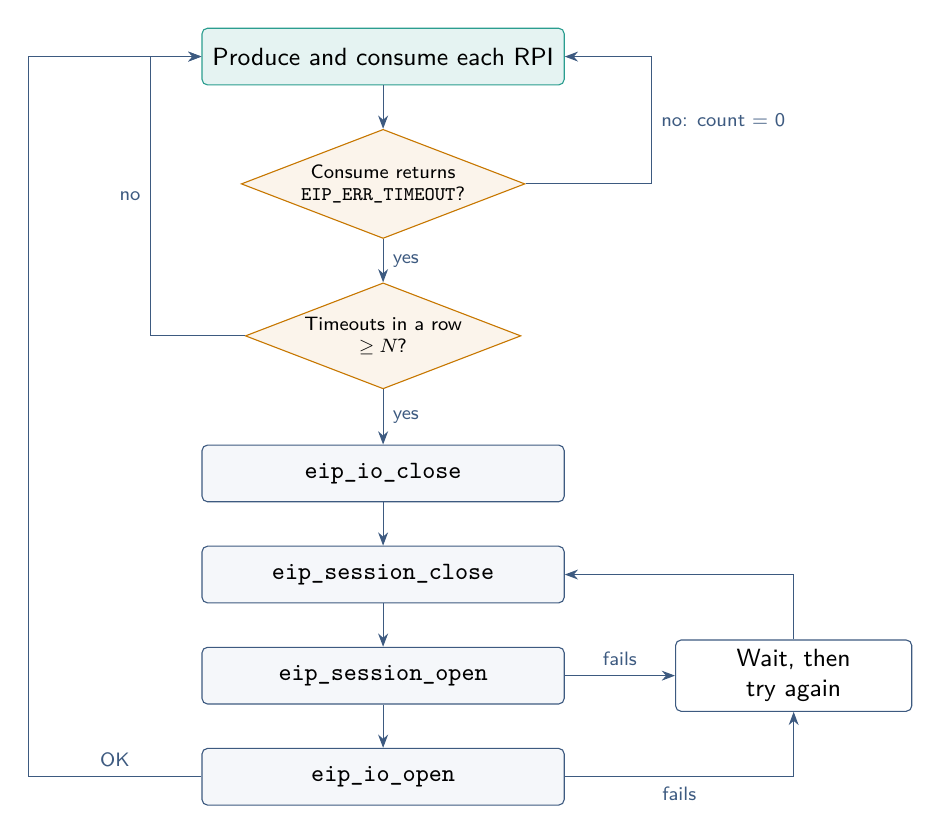
\begin{tikzpicture}[
  font=\sffamily\small,>=Stealth,node distance=0.55cm,
  stp/.style={draw=steel,fill=white,rounded corners=2pt,minimum width=4.6cm,minimum height=0.72cm,align=center},
  call/.style={stp,fill=codebg,font=\ttfamily\small},
  dec/.style={diamond,aspect=2.6,draw=amber,fill=amber!8,inner sep=1pt,align=center,font=\sffamily\scriptsize},
  lab/.style={font=\sffamily\scriptsize,text=steel}]
  \node[stp,fill=teal!12,draw=teal] (loop) {Produce and consume each RPI};
  \node[dec,below=of loop] (to) {Consume returns\\\code{EIP_ERR_TIMEOUT}?};
  \node[dec,below=of to] (n) {Timeouts in a row\\$\geq N$?};
  \node[call,below=0.7cm of n] (c1) {eip\_io\_close};
  \node[call,below=of c1] (c2) {eip\_session\_close};
  \node[call,below=of c2] (c3) {eip\_session\_open};
  \node[call,below=of c3] (c4) {eip\_io\_open};
  \node[stp,right=1.4cm of c3,minimum width=3.0cm] (wait) {Wait, then\\try again};
  \draw[->,steel] (loop) -- (to);
  \draw[->,steel] (to) -- node[lab,right]{yes} (n);
  \draw[->,steel] (to.east) -- ++(1.6,0) |- node[lab,pos=0.25,right]{no: count = 0} (loop.east);
  \draw[->,steel] (n.west) -- ++(-1.2,0) |- node[lab,pos=0.25,left]{no} (loop.west);
  \draw[->,steel] (n) -- node[lab,right]{yes} (c1);
  \draw[->,steel] (c1) -- (c2);
  \draw[->,steel] (c2) -- (c3);
  \draw[->,steel] (c3) -- (c4);
  \draw[->,steel] (c3.east) -- node[lab,above]{fails} (wait.west);
  \draw[->,steel] (wait.north) |- (c2.east);
  \draw[->,steel] (c4.west) -- ++(-2.2,0) node[lab,above,pos=0.5]{OK} |- (loop.west);
  \draw[->,steel] (c4.east) -| node[lab,below,pos=0.25]{fails} (wait.south);
\end{tikzpicture}
\caption{Recovery of a lost Class~1 connection on the originator. The four
calls are all necessary: a reopen of I/O on the old session fails.}
\label{fig:recover}
\end{figure}

\begin{procedure}{Recover a lost Class 1 connection}
\begin{enumerate}
  \item Count the calls to \code{eip_io_consume} in a row that return
        \code{EIP_ERR_TIMEOUT}.
  \item When the count gets to your limit, call \code{eip_io_close}.
  \item Call \code{eip_session_close}.
  \item Call \code{eip_session_open}.
  \item If the open fails, wait and do step 3 again.
  \item Call \code{eip_io_open}.
  \item Set the count to 0, and start the produce and consume loop again.
\end{enumerate}
\end{procedure}

\begin{note}
\notelabel When the peer is gone, \code{eip_io_close} can block for the session
timeout and return an error. This is the expected result. The call still
releases the UDP socket.
\end{note}

If you do not close and open the session, \code{eip_io_open} returns
\code{EIP_ERR_IO}.

\chapter{Platform Integration}\label{ch:platforms}

This chapter gives the steps to add QuickEIP to a project on each shipped
platform. Table~\ref{tab:platforms} gives the test status of each port.

% -------------------------------------------------------------------------
\section{NetBurner NNDK}\label{sec:netburner}

The port was tested with NNDK 3.5.8 on ARM platforms. The NNDK 3.x socket
API is the same on all platforms.

\begin{procedure}{Add QuickEIP to an NNDK project}
\begin{enumerate}
  \item Put QuickEIP in a subdirectory of the project, for example
        \file{MyProject/QuickEIP}. A git submodule is also correct.
  \item Write the makefile of the project (listing below).
  \item Set the NNDK environment variables.
  \item Run \code{make}.
  \item Find the image at \file{obj/release/MyProject.bin}.
\end{enumerate}
\end{procedure}

\begin{note}
\notelabel The NNDK rules put each object file at
\file{obj/release/}\textit{source path}. A source path that starts with
\file{../} thus puts the object files outside \file{obj/}, next to your
sources. Keep QuickEIP inside the project directory to prevent this.
\end{note}

This is a complete makefile, with QuickEIP in a subdirectory:

\begin{lstlisting}[language=make]
NAME    = MyProject

CPP_SRC += src/main.cpp

QUICKEIP = QuickEIP

C_SRC   += $(QUICKEIP)/src/eip_codec.c \
           $(QUICKEIP)/src/eip_adapter.c \
           $(QUICKEIP)/src/eip_session.c \
           $(QUICKEIP)/src/eip_io.c \
           $(QUICKEIP)/src/eip_scan.c \
           $(QUICKEIP)/src/eip_server.c \
           $(QUICKEIP)/src/eip_adapter_default.c
CPP_SRC += $(QUICKEIP)/ports/netburner/eip_hal_netburner.cpp
NBINCLUDE += -I$(QUICKEIP)/include -I$(QUICKEIP)/src

include $(NNDK_ROOT)/make/boilerplate.mk
\end{lstlisting}

Set the environment and build, for example:

\begin{lstlisting}[language=shell]
export NNDK_ROOT=C:/nburn PLATFORM=MODM7AE70 DEFPLATFORM=MODM7AE70
export PATH=/c/nburn/gcc/bin:/c/nburn/pcbin:/c/nburn/gcc/msys/1.0/bin:$PATH
make
\end{lstlisting}

The first build takes several minutes, because the NNDK compiles its system
library into the \file{obj/} directory of the project. This is normal. For
NBEclipse, add the same files to the project. Add the two include directories
to the C and the C++ compiler settings.

\subsection{Start QuickEIP from UserMain}

Scanner calls block, so run them in a task of their own. Each task needs its
own priority, and a lower number runs first. The adapter task uses
\code{MAIN_PRIO - 1}. Thus \code{MAIN_PRIO + 1} is a safe priority for the
scanner task. \code{UserMain} must then sleep, so that the scanner task can
run.

\begin{lstlisting}[language=C++]
#include <init.h>
#include <nbrtos.h>
#include <string.h>

#include "eip.h"

const char *AppName = "MyProject";

static void ScannerTask(void *)
{
    for (;;) {
        /* eip_session_open, eip_tag_read, and so on (chapter 6) */
        OSTimeDly(TICKS_PER_SECOND);
    }
}

void UserMain(void *)
{
    EipAdapterConfig cfg;

    init();
    WaitForActiveNetwork(TICKS_PER_SECOND * 10);

    memset(&cfg, 0, sizeof cfg);
    /* fill in cfg as in chapter 4 */
    eip_adapter_start(&cfg);
    OSSimpleTaskCreatewName(ScannerTask, MAIN_PRIO + 1, "EipScanner");

    for (;;) {
        /* eip_adapter_read and eip_adapter_write */
        OSTimeDly(1);
    }
}
\end{lstlisting}

\subsection{Platform Notes}

\begin{description}[font=\sffamily\bfseries\color{steel}]
  \item[Clock resolution.] \code{eip_hal_millis} follows \code{TimeTick}: 50~ms
        at the default 20~Hz. The adapter never sets a Class~1 timeout shorter
        than two ticks (100~ms), and \TO{} packets go out on tick boundaries.
        For RPIs shorter than approximately 50~ms, increase
        \code{TICKS_PER_SECOND} in the platform configuration.
  \item[Task.] The adapter task runs at \code{MAIN_PRIO - 1} by default. Set
        \code{EIP_ADAPTER_TASK_PRIORITY} to change it. The task uses the
        default NNDK task stack.
  \item[Lock.] \code{eip_hal_lock} is \code{OSLock()}, which stops task
        switches for a short time. It is never held during a socket call.
  \item[UDP sockets.] The port uses \code{CreateRxTxUdpSocket4} with an
        explicit local port. When the library asks for ``any port,'' the port
        selects one in 50000--50063.
  \item[TCP options.] The port does not set TCP\_NODELAY or keep-alive. A slot
        of a lost peer comes back through eviction after
        \code{EIP_ADAPTER_EVICT_MS}.
  \item[Web UI.] \file{examples/netburner_webui} is a test web page. It is
        application code, not part of the stack. It has no \code{main} and no
        makefile, so add it to an NNDK application.
\end{description}

% -------------------------------------------------------------------------
\section{ESP-IDF (ESP32)}\label{sec:espidf}

The port was tested with ESP-IDF 5.5.1 on the esp32 target. All ESP-IDF 5.x
versions should operate.

\subsection{Add the Component}

The root directory of QuickEIP is an IDF component. The component takes the
name of its directory. Use the same spelling in all locations. The simpler
method is a top-level \file{CMakeLists.txt} that names the directory. The
path is relative to the project. Here QuickEIP is beside it:

\begin{lstlisting}[language=cmake]
cmake_minimum_required(VERSION 3.16)
list(APPEND EXTRA_COMPONENT_DIRS "${CMAKE_CURRENT_LIST_DIR}/../QuickEIP")
include($ENV{IDF_PATH}/tools/cmake/project.cmake)
project(myapp)
\end{lstlisting}

With the component manager, put the dependency in \file{main/idf_component.yml}.
The path is relative to \file{main/}:

\begin{lstlisting}[language=yaml]
dependencies:
  QuickEIP:
    path: ../../QuickEIP
\end{lstlisting}

\begin{caution}
The dependency key must be the same as the directory name. If it is not, the
build fails with \code{Failed to resolve component ... unknown name}. A change
to \code{REQUIRES} does not correct this error.
\end{caution}

With the two methods, \file{main/CMakeLists.txt} names the component and the
network components that you use:

\begin{lstlisting}[language=cmake]
idf_component_register(SRCS "main.c"
                       INCLUDE_DIRS "."
                       REQUIRES QuickEIP esp_eth esp_netif esp_event)
\end{lstlisting}

Build with \code{idf.py set-target esp32} and then \code{idf.py build}.

\subsection{Start Ethernet}

Use the driver code in \file{examples/ethernet/basic} of ESP-IDF as a model.

\begin{warning}
You must know the PHY, the pins, and the RMII clock mode of your board. A
wrong value compiles without an error, but the link never comes up. Get these
values from the schematic of the board. Do not guess them.
\end{warning}

This example is for the internal EMAC of the ESP32 with a LAN87xx PHY:

\begin{lstlisting}
#include "esp_eth.h"
#include "esp_event.h"
#include "esp_netif.h"

static esp_eth_handle_t s_eth;
static esp_netif_t *s_netif;
static volatile int s_link_up;

static void eth_event(void *arg, esp_event_base_t base, int32_t id, void *data)
{
    (void)arg; (void)base; (void)data;
    if (id == ETHERNET_EVENT_CONNECTED) s_link_up = 1;
    else if (id == ETHERNET_EVENT_DISCONNECTED) s_link_up = 0;
}

static void eth_start(void)
{
    eth_mac_config_t mac_cfg = ETH_MAC_DEFAULT_CONFIG();
    eth_esp32_emac_config_t emac_cfg = ETH_ESP32_EMAC_DEFAULT_CONFIG(); /* set smi_gpio and clock_config */
    eth_phy_config_t phy_cfg = ETH_PHY_DEFAULT_CONFIG();                /* and your PHY address */
    esp_eth_mac_t *mac = esp_eth_mac_new_esp32(&emac_cfg, &mac_cfg);
    esp_eth_phy_t *phy = esp_eth_phy_new_lan87xx(&phy_cfg);
    esp_eth_config_t eth_cfg = ETH_DEFAULT_CONFIG(mac, phy);
    esp_netif_config_t netif_cfg = ESP_NETIF_DEFAULT_ETH();

    ESP_ERROR_CHECK(esp_eth_driver_install(&eth_cfg, &s_eth));
    ESP_ERROR_CHECK(esp_netif_init());
    ESP_ERROR_CHECK(esp_event_loop_create_default());
    s_netif = esp_netif_new(&netif_cfg);
    ESP_ERROR_CHECK(esp_netif_attach(s_netif, esp_eth_new_netif_glue(s_eth)));
    ESP_ERROR_CHECK(esp_event_handler_register(ETH_EVENT, ESP_EVENT_ANY_ID, eth_event, NULL));
    ESP_ERROR_CHECK(esp_eth_start(s_eth));
}
\end{lstlisting}

\subsection{Report the Link}

The esp\_netif layer does not report speed or duplex. Read them from the
driver in a \code{link_info} callback. Return 1 while the link is up, and 0 to
report it down:

\begin{lstlisting}
static int link_info(void *ctx, uint32_t *mbps, int *full, int *autoneg)
{
    eth_speed_t speed;
    eth_duplex_t duplex;
    (void)ctx;
    if (!s_link_up) return 0;
    if (esp_eth_ioctl(s_eth, ETH_CMD_G_SPEED, &speed) != ESP_OK) return 0;
    if (esp_eth_ioctl(s_eth, ETH_CMD_G_DUPLEX_MODE, &duplex) != ESP_OK) return 0;
    *mbps = (speed == ETH_SPEED_100M) ? 100 : 10;
    *full = (duplex == ETH_DUPLEX_FULL);
    *autoneg = 1;
    return 1;
}
\end{lstlisting}

\subsection{Start the Adapter}

\begin{procedure}{Start the adapter on ESP-IDF}
\begin{enumerate}
  \item Call \code{eth_start}.
  \item Set all fields of \code{cfg} (chapter~\ref{ch:adapter}).
  \item Set \code{cfg.link_info} to your callback.
  \item Optional: call \code{eip_esp_set_netif} to select the interfaces.
  \item Call \code{eip_adapter_start}.
\end{enumerate}
\end{procedure}

\begin{lstlisting}
#include "eip.h"
#include "eip_esp_idf.h"

eth_start();
cfg.link_info = link_info;       /* with the rest of cfg, from chapter 4 */
eip_esp_set_netif(&s_netif, 1);  /* optional: default is ETH_DEF, WIFI_STA_DEF, WIFI_AP_DEF */
eip_adapter_start(&cfg);
\end{lstlisting}

Call \code{eip_esp_set_netif} before \code{eip_adapter_start}. The function
copies the list, and the netifs must stay valid while the adapter runs.

\subsection{Options}

Put the options in compile definitions for all components. In the top-level
\file{CMakeLists.txt}, set them after the line that includes
\file{project.cmake} and before \code{project()}:

\begin{lstlisting}[language=cmake]
idf_build_set_property(COMPILE_DEFINITIONS "EIP_ESP_TASK_PRIORITY=12" APPEND)
idf_build_set_property(COMPILE_DEFINITIONS "EIP_ESP_TASK_WDT=1" APPEND)
\end{lstlisting}

\begin{table}[htbp]
\centering
\caption{ESP-IDF port options}\label{tab:espopts}
\begin{tabularx}{\linewidth}{@{}P{0.30\linewidth}P{0.17\linewidth}L@{}}
\toprule
\textbf{Define} & \textbf{Default} & \textbf{Effect} \\
\midrule
\code{EIP_ESP_TASK_STACK} & 6144 & Adapter task stack in bytes (or \code{EIP_ADAPTER_TASK_STACK}). \\
\code{EIP_ESP_TASK_PRIORITY} & 12 & Adapter task priority (or \code{EIP_ADAPTER_TASK_PRIORITY}). \\
\code{EIP_ESP_TASK_CORE} & \code{tskNO_AFFINITY} & Pins the adapter task to a core. \\
\code{EIP_ESP_TASK_WDT} & 0 & 1 adds the adapter task to the task watchdog. \\
\bottomrule
\end{tabularx}
\end{table}

\subsection{Platform Notes}

\begin{itemize}
  \item Use wired Ethernet for Class~1 in production. Wi-Fi latency peaks are
        frequently longer than a timeout of 8 $\times$ RPI.
  \item The adapter task waits in \code{select()}, so it starts as soon as a
        packet arrives. While idle, it still does a pass at least each
        \code{EIP_ADAPTER_IDLE_WAIT_MS} (5~ms).
  \item Arduino-ESP32 runs on ESP-IDF and can use the same files. Make a
        library directory whose \file{src/} contains \file{include/*},
        \file{src/*}, \file{ports/bsd_sockets/*}, and \file{ports/esp-idf/*}.
        Do not include the other ports, because Arduino compiles all files
        that it finds. This setup has not been tested.
  \item The example \file{examples/esp_idf_adapter} uses
        \code{protocol_examples_common}. For that example only, run
        \code{idf.py menuconfig} and set the network under
        \menu{Example Connection Configuration}.
\end{itemize}

% -------------------------------------------------------------------------
\section{Teknic ClearCore}\label{sec:clearcore}

\file{examples/clearcore_adapter} compiles and links with the arm-gcc 6.3 of
Microchip Studio, against the Enhanced ClearCore Library, a fork of ClearCore
library 1.7. The adapter has run on a ClearCore with a Micro850 PLC. The
example itself has not been run.

ClearCore runs on bare metal (no RTOS), on the raw API of lwIP with
\code{NO_SYS=1}. QuickEIP uses lwIP directly through \file{ports/lwip_raw}. It
does not use the \code{EthernetTcp*} and \code{EthernetUdp} classes. Those
classes have a 600-byte TCP buffer and no broadcast send, and EtherNet/IP
needs more.

\begin{procedure}{Set up a ClearCore project}
\begin{enumerate}
  \item Copy \file{ProjectTemplate}, \file{libClearCore}, and \file{LwIP}
        from the ClearCore library directory to a location where you can
        write.
  \item Put your QuickEIP directory beside them. The four directories must be
        at the same level, because the paths below are relative.
  \item Open \file{ProjectTemplate.atsln}.
  \item Make sure that the three projects load.
  \item Add the files with \menu{Add $\to$ Existing Item $\to$ Add As Link}:
        \file{src/*.c} (all files), \file{ports/lwip_raw/eip_hal_lwip_raw.c},
        and \file{ports/clearcore/eip_hal_clearcore.cpp}.
  \item Open \menu{Project Properties $\to$ Toolchain}. Do steps 7--10 in the
        Debug and the Release configurations.
  \item In \menu{ARM/GNU C Compiler $\to$ Directories} and \menu{ARM/GNU C++
        Compiler $\to$ Directories}, add \file{../../QuickEIP/include} and
        \file{../../QuickEIP/src}.
  \item In \menu{ARM/GNU C Compiler $\to$ Directories} only, add
        \file{../../LwIP/LwIP/src/include} and
        \file{../../LwIP/LwIP/port/include}.
  \item In \menu{ARM/GNU C Compiler $\to$ Symbols} and \menu{ARM/GNU C++
        Compiler $\to$ Symbols}, add \code{EIP_ADAPTER_MAX_CLIENTS=2}.
  \item Keep the symbols \code{DEBUG} and \code{NDEBUG} and the flag
        \code{-std=gnu11} that are in the template.
  \item Replace \file{main.cpp} of the template with your main loop.
\end{enumerate}
\end{procedure}

\begin{note}
\notelabel The template sets the lwIP include paths for C++ only. The lwIP
port is a C file. Without step 8, the build stops at \file{lwip/ip_addr.h}.
\end{note}

\begin{caution}
Add \code{EIP_ADAPTER_MAX_CLIENTS=2} to the C and the C++ symbols. It changes
the size of structures, so the two compilers must agree. The default of 4 is
too many for this lwIP build.
\end{caution}

Paths are relative to the \file{Debug} or \file{Release} output directory.
To check a compile without Studio, run \code{arm-none-eabi-gcc} or
\code{arm-none-eabi-g++} with \code{-c} from \file{ProjectTemplate/Debug} and
these flags. The toolchain is in
\file{Atmel/Studio/7.0/toolchain/arm/arm-gnu-toolchain/bin}, and
\textit{Packs} is \file{Atmel/Studio/7.0/Packs}:

\begin{lstlisting}[language=shell]
-mthumb -mcpu=cortex-m4 -mfloat-abi=hard -mfpu=fpv4-sp-d16
-D__SAME53N19A__ -DEIP_ADAPTER_MAX_CLIENTS=2
-I../../QuickEIP/include -I../../QuickEIP/src -I../../QuickEIP/ports/clearcore
-I../../libClearCore/inc -I../../LwIP/LwIP/src/include -I../../LwIP/LwIP/port/include
-I<Packs>/atmel/SAME53_DFP/1.1.118/include
-I<Packs>/arm/CMSIS/4.5.0/CMSIS/Include
-I<Packs>/arm/CMSIS/5.4.0/CMSIS/Core/Include
\end{lstlisting}

\subsection{The Main Loop}

The full example is in \file{examples/clearcore_adapter/main.cpp}:

\begin{lstlisting}[language=C++]
#include "ClearCore.h"
#include "eip.h"

while (!EthernetMgr.PhyLinkActive()) {                 // wait for the cable
    Delay_ms(100);
}
EthernetMgr.Setup();
if (!EthernetMgr.DhcpBegin()) {
    EthernetMgr.LocalIp(IpAddress(192, 168, 1, 50));   // fallback static address
}
if (eip_adapter_start(&cfg) != EIP_OK) {               // poll mode: starts no task
    while (true) { EthernetMgr.Refresh(); }            // stop: outputs stay off
}

while (true) {
    eip_adapter_poll();             // every pass
    EthernetMgr.Refresh();
    // motion, I/O, eip_adapter_read / eip_adapter_write ...
}
\end{lstlisting}

\subsection{Platform Notes}

\begin{description}[font=\sffamily\bfseries\color{steel}]
  \item[Call \code{eip_adapter_poll} frequently.] \TO{} packets go out from
        inside the poll call. Thus the loop time becomes RPI jitter. Keep the
        loop time much shorter than your RPI.
  \item[The lwIP build is small.] It has a 4~KB heap (\code{MEM_SIZE}), five
        TCP PCBs, and eight listening PCBs. The adapter uses one listening PCB
        plus one PCB for each explicit session. A scanner session uses one
        more. This is why you set \code{EIP_ADAPTER_MAX_CLIENTS} to 2 or 3. For
        more, compile the LwIP project again with a larger \code{MEM_SIZE} and
        \code{MEMP_NUM_TCP_PCB}. Its \file{lwipopts.h} uses \code{\#ifndef},
        so \code{-D} operates.
  \item[Blocking scanner calls.] They call \code{EthernetMgr.Refresh()} while
        they wait, and motion continues from interrupts. But your main loop
        does not run until the call returns. Keep \code{timeout_ms} short.
  \item[Interrupts.] Do not call QuickEIP from an interrupt handler. The lwIP
        callbacks run inside \code{EthernetMgr.Refresh()} in the main context.
        This is why the port needs no lock.
  \item[Socket table.] \code{EIP_LWIP_MAX_SOCKETS} (12),
        \code{EIP_LWIP_UDP_QUEUE} (8), and \code{EIP_LWIP_ACCEPT_QUEUE} (4) set
        the size of the raw-API socket table.
  \item[Link report.] The port reports 100~Mbit/s full duplex while the PHY
        link is up.
  \item[Multicast \TO.] The port sets TTL 1 only in lwIP builds with
        \code{LWIP_MULTICAST_TX_OPTIONS}. The standard build does not have
        this option. Thus use a point-to-point connection.
  \item[Host name.] lwIP on ClearCore has no host name. Call
        \code{eip_clearcore_set_host_name} at start-up, and again from
        \code{apply_interface} when a scanner sets attribute 6.
\end{description}

\begin{warning}
On ClearCore, the main loop also controls motion. A blocking scanner call
stops the main loop until it returns. Do not make scanner calls while motion
needs service from the main loop. Keep \code{timeout_ms} short.
\end{warning}

The same three groups of files should also operate as an Arduino library with
the ClearCore wrapper. This has not been tested.

% -------------------------------------------------------------------------
\section{Linux, macOS, and WSL}\label{sec:posix}

Section~\ref{sec:hostbuild} gives the build procedure. The build makes
\file{libquickeip.a} (the core and the POSIX port), the tests, and
\code{eiptool}. Appendix~\ref{app:tools} describes \code{eiptool}.

\begin{itemize}
  \item Set \code{EIP_NETIF=eth1} to select the interface that the adapter
        reports and that the scan uses first. This applies to all programs that
        use the POSIX port. The port ignores an unknown name and uses the
        default interface.
  \item Ports 44818 and 2222 are above 1024, so you do not need root access.
        Another EtherNet/IP program on the same host blocks them.
  \item Under WSL2, the host is behind NAT. A scan to the LAN operates, but
        PLCs on your LAN cannot get to a WSL adapter. Use mirrored networking.
\end{itemize}

% -------------------------------------------------------------------------
\section{Windows}\label{sec:windows}

The port was tested with Visual Studio 2022 on Windows 11, as x64 and Win32.
The port is \file{ports/windows/eip_hal_windows.c}. It needs Windows 7 or
later. Section~\ref{sec:hostbuild} gives the build procedure.

\begin{procedure}{Add QuickEIP to a Windows project}
\begin{enumerate}
  \item Compile \file{src/*.c} and \file{ports/windows/eip_hal_windows.c}.
  \item Add \file{include/} and \file{src/} to the include path.
  \item Link \code{ws2_32}, \code{iphlpapi}, and \code{winmm}.
\end{enumerate}
\end{procedure}

\begin{table}[htbp]
\centering
\caption{Windows port options}\label{tab:winopts}
\small
\begin{tabularx}{\linewidth}{@{}P{0.32\linewidth}P{0.10\linewidth}L@{}}
\toprule
\textbf{Define} & \textbf{Default} & \textbf{Effect} \\
\midrule
\code{EIP_WIN_POLL_MODE} & Off & Starts no adapter thread. Your loop calls \code{eip_adapter_poll}. \\
\code{EIP_ADAPTER_TASK_PRIORITY} & 0 & A \code{THREAD_PRIORITY_*} value for the adapter thread. 0 selects \code{THREAD_PRIORITY_HIGHEST}. \\
\code{EIP_ADAPTER_TASK_STACK} & 0 & Adapter thread stack in bytes. 0 is the system default. \\
\code{EIP_WIN_MAX_SOCKETS} & 64 & Sockets open at the same time. \\
\code{EIP_WIN_MAX_INTERFACES} & 16 & Interfaces reported. \\
\code{EIP_WIN_NETIF_REFRESH_MS} & 2000 & Interval at which the port reads the interface list again, outside the adapter thread. \\
\bottomrule
\end{tabularx}
\end{table}

\subsection{Platform Notes}

\begin{description}[font=\sffamily\bfseries\color{steel}]
  \item[Select the interface on a PC with more than one.] The adapter reports
        interface 0 as its address, in ListIdentity and in the \OT{} socket
        address of a Forward\_Open. Interface 0 is the first one that is up
        and has a default gateway. Frequently, this is not the machine
        network. Set \code{EIP_NETIF} to the friendly name or the IPv4 address
        of the adapter interface, for example \code{EIP_NETIF="Ethernet 2"} or
        \code{EIP_NETIF=10.168.41.1}. The port keeps a named interface also
        while its cable is disconnected, and reports the link as down. Scanner
        calls do not need this setting.
  \item[Firewall.] An adapter needs inbound TCP 44818, UDP 44818, and UDP
        2222 for your program. A scanner that runs Class~1 needs inbound UDP
        on its local port. Use \code{Get-NetConnectionProfile} to find the
        profile of the network.
  \item[A new executable can lose its first replies.] Third-party security
        software can stop inbound UDP for the first seconds that a new
        program runs, also with Windows Firewall off. On a test PC with AVG,
        each new binary failed its first \code{eiptool identity}, and then
        answered in approximately 45~ms. If a new build times out, or a scan
        finds too few devices, run it again before you look for a network
        fault.
  \item[Busy ports.] Other EtherNet/IP software on the PC, such as RSLinx,
        can hold 44818 or 2222. Each bind is exclusive. The adapter then
        cannot open the ports, and \code{listening} stays 0.
  \item[Timing.] The port sets a 1~ms system timer period for the process
        from its first call. This uses more power on a laptop. On the test PC,
        a 10~ms RPI had a mean of 10.00~ms and a maximum of 11.83~ms over
        \num{1500} packets, with the two ends on the same host.
  \item[Link report.] Windows gives the speed. It does not give duplex or
        autonegotiation, so the port reports full duplex and autonegotiated
        while the link is up.
  \item[Not tested.] Multicast \TO, and a real PLC connected to a Windows
        adapter.
\end{description}

\begin{warning}
Windows is not a real-time operating system. A stall of approximately 100~ms
was measured on a bench PC. Set \code{timeout_floor_ms} to 500 or more. Do
not use a Windows adapter for a safety function.
\end{warning}

\chapter{Porting to a New Platform}\label{ch:porting}

A port is one source file, sometimes two, that implements the functions in
\file{include/eip_hal.h}. The core calls these functions directly. There is
no function table. This chapter tells you what each function must do and how
to check a new port.

\section{Select a Starting Point}

Start from the port that is nearest to your platform.
Table~\ref{tab:portstart} shows which port to use.

\begin{table}[htbp]
\centering
\caption{Starting points for a new port}\label{tab:portstart}
\small
\begin{tabularx}{\linewidth}{@{}P{0.32\linewidth}P{0.30\linewidth}L@{}}
\toprule
\textbf{Your platform has} & \textbf{Start from} & \textbf{You write} \\
\midrule
BSD sockets (\code{socket}, \code{select}, \code{fcntl}): lwIP with \code{LWIP_SOCKET}, Zephyr, Linux, FreeRTOS+TCP with its BSD layer & \file{ports/bsd_sockets/eip_hal_bsd_sockets.c}, without changes & A platform file like \file{ports/esp-idf/eip_hal_esp_idf.c}: clock, lock, interfaces, and task \\
The lwIP raw API, \code{NO_SYS=1}, no socket layer: STM32Cube bare metal, SAM, other boards like ClearCore & \file{ports/lwip_raw/eip_hal_lwip_raw.c}, without changes & A platform file like \file{ports/clearcore/eip_hal_clearcore.cpp}: clock, yield (your stack poll), and interfaces \\
A vendor socket API that is neither (NetBurner) & \file{ports/netburner/eip_hal_netburner.cpp} & The full contract \\
Winsock & \file{ports/windows/eip_hal_windows.c}, without changes & Nothing \\
\bottomrule
\end{tabularx}
\end{table}

The platform file is short. For ESP-IDF it is approximately 190 lines with
comments, and for ClearCore approximately 130.

\section{General Rules of the Contract}

\begin{description}[font=\sffamily\bfseries\color{steel}]
  \item[Handles.] A socket handle is an \code{int}. A negative value is not
        valid, and \code{EIP_SOCK_INVALID} is $-1$. The core records which
        handles it owns, so 0 is a valid handle.
  \item[Addresses.] An IPv4 address is \code{uint8_t[4]} in network order,
        for example \code{\{192,168,1,10\}}. A port number is a plain integer
        in host order.
  \item[Timeouts.] \code{timeout_ms == 0} means ``do not wait.'' Return what
        is ready now.
  \item[Blocking waits.] Each blocking wait must keep the network stack in
        operation. On bare metal, call the stack poll inside the loop. This is
        the purpose of \code{eip_hal_yield}.
  \item[Return codes.] \code{EIP_OK} (0) or a negative \code{EIP_ERR_*},
        unless the function gives a different rule.
\end{description}

\section{Time and Scheduling}

\begin{table}[htbp]
\centering
\caption{Port functions: time, scheduling, and lock}\label{tab:halttime}
\small
\begin{tabularx}{\linewidth}{@{}P{0.34\linewidth}L@{}}
\toprule
\textbf{Function} & \textbf{Must} \\
\midrule
\code{eip_hal_millis} & Return a free-running millisecond counter that wraps at $2^{32}$. The core uses only differences. \TO{} packets are timed from it, so use a real 1~ms source if the platform has one. \\
\code{eip_hal_clock_resolution_ms} & Return the real step of the counter in milliseconds (1 for a 1~kHz source). The adapter never sets a Class~1 timeout shorter than two steps. \\
\code{eip_hal_yield} & Let other work run for a short time. On an RTOS, sleep one tick. On bare metal, run the poll of the network stack, for example \code{EthernetMgr.Refresh()}, or \code{sys_check_timeouts()} plus \code{ethernetif_input()}. \\
\code{eip_hal_lock}, \code{eip_hal_unlock} & Give mutual exclusion between the adapter context and application tasks. The lock is not nested, is held for microseconds, and is never held during a socket call. The core can read \code{eip_hal_millis} while it holds the lock. Single-threaded ports leave the two functions empty. \\
\bottomrule
\end{tabularx}
\end{table}

\begin{caution}
Use a clock with a real 1~ms step if the platform has one. On Windows,
\code{GetTickCount64} steps approximately each 16~ms. With that clock, the
adapter sent \TO{} at approximately half the rate, and the connection timed
out. \file{tests/test_hal.c} measures the step and fails a clock that is
coarser than it reports.
\end{caution}

\section{Network Interfaces}

\code{eip_hal_netif_get(index, info)} fills in the data of interface
\code{index}. Index 0 is the primary interface. These rules apply:

\begin{itemize}
  \item Return \code{EIP_ERR_ARG} after the last interface.
  \item An interface without an address still returns \code{EIP_OK}, with
        \code{ip} = 0.0.0.0. The POSIX port is an exception. It lists only
        interfaces that are up and have an IPv4 address.
  \item Set to zero all fields that you do not know.
  \item Set \code{link_known = 1} when you can report \code{link_up}. If you
        do not, the server uses ``has an address'' as ``link up, 100~Mbit/s
        full duplex.'' Fill \code{speed_mbps}, \code{full_duplex}, and
        \code{autonegotiated} with real values if you can.
\end{itemize}

The core uses the result in three ways:

\begin{enumerate}
  \item The adapter calls the function each 100~ms for \code{netif_index}. It
        fills in its Identity, TCP/IP Interface, and Ethernet Link objects.
  \item The scan reads indexes 0, 1, 2, and so on, to find broadcast addresses.
  \item The MAC address sets the default serial number.
\end{enumerate}

\section{TCP}

\begin{table}[htbp]
\centering
\caption{Port functions: TCP}\label{tab:haltcp}
\small
\begin{tabularx}{\linewidth}{@{}P{0.30\linewidth}L@{}}
\toprule
\textbf{Function} & \textbf{Must} \\
\midrule
\code{eip_hal_tcp_connect} & Connect, and wait up to \code{timeout_ms}. Return a handle or \code{EIP_SOCK_INVALID}. \\
\code{eip_hal_tcp_listen} & Listen on all addresses. Return a handle or \code{EIP_SOCK_INVALID}. \\
\code{eip_hal_tcp_accept} & \textbf{Never block.} Return a connected handle and fill \code{peer_ip}, or return \code{EIP_SOCK_INVALID} when no client waits. \\
\code{eip_hal_tcp_send} & Queue \textbf{all} \code{len} bytes. Return \code{EIP_ERR_IO} if the connection is broken, or if the bytes cannot be queued in a few hundred milliseconds. Do not block for an unlimited time. \\
\code{eip_hal_tcp_recv} & Return the number of bytes read ($>0$), 0 if nothing arrived in time, or \code{EIP_ERR_IO} after the peer closed or the connection failed. With \code{timeout_ms == 0}, return immediately. \\
\code{eip_hal_tcp_local_ip} & Return the local address of the connection. It goes into the \TO{} socket address of a Forward\_Open. \\
\code{eip_hal_tcp_close} & Close the socket and release the handle. This applies to connected and listening sockets. \\
\bottomrule
\end{tabularx}
\end{table}

For adapter sessions, set TCP\_NODELAY and keep-alive (approximately 30~s
idle, three probes). Table~\ref{tab:tcpopts} shows what the shipped ports do.

\begin{table}[htbp]
\centering
\caption{TCP options in the shipped socket layers}\label{tab:tcpopts}
\small
\begin{tabularx}{\linewidth}{@{}P{0.18\linewidth}P{0.22\linewidth}L@{}}
\toprule
\textbf{Layer} & \textbf{TCP\_NODELAY} & \textbf{Keep-alive} \\
\midrule
\file{bsd_sockets} & All connections & Accepted sockets only. The 30~s setting needs \code{TCP_KEEPIDLE}, \code{TCP_KEEPINTVL}, and \code{TCP_KEEPCNT}. \\
\file{lwip_raw} & All connections & Only in lwIP builds with \code{LWIP_TCP_KEEPALIVE}. \\
\file{netburner} & No & No. The slot of a lost peer comes back through eviction. \\
\bottomrule
\end{tabularx}
\end{table}

\section{UDP}

\begin{table}[htbp]
\centering
\caption{Port functions: UDP}\label{tab:haludp}
\small
\begin{tabularx}{\linewidth}{@{}P{0.30\linewidth}L@{}}
\toprule
\textbf{Function} & \textbf{Must} \\
\midrule
\code{eip_hal_udp_open} & Bind on all addresses. \code{local_port == 0} means any free port. \textbf{Fail if the port is already in use.} \code{EIP_UDP_BROADCAST} permits broadcast sends. \code{EIP_UDP_MULTICAST_TX} permits multicast sends with TTL 1 on the primary interface, where the stack can set them. \\
\code{eip_hal_udp_sendto} & Send one datagram. Return \code{EIP_OK} or \code{EIP_ERR_IO}. \\
\code{eip_hal_udp_recvfrom} & Receive one datagram. Return its length, 0 if nothing arrived in time, or \code{EIP_ERR_IO}. Cut a long datagram to \code{cap}. \code{ip} and \code{port} can be null. \\
\code{eip_hal_udp_close} & Close the socket and release the handle. \\
\bottomrule
\end{tabularx}
\end{table}

\begin{caution}
Do not use \code{SO_REUSEADDR}. The scanner finds a free port in UDP
2223--2231 because a bind to a port in use fails. The same failure stops an
explicit \code{local_port} of 2222 while an adapter runs on the same device.
\end{caution}

A socket bound to the any-address must receive broadcasts. The adapter
answers broadcast ListIdentity requests on UDP 44818.

\section{Wait and the Adapter Runner}

\begin{table}[htbp]
\centering
\caption{Port functions: wait and runner}\label{tab:halrun}
\small
\begin{tabularx}{\linewidth}{@{}P{0.30\linewidth}L@{}}
\toprule
\textbf{Function} & \textbf{Must} \\
\midrule
\code{eip_hal_wait} & Wait until one of the handles can be readable (or a listener has a connection), or until the timeout. Skip handles that are not valid. The function can return early. Without \code{select()}, a loop of \code{eip_hal_yield} and readiness checks is correct. \\
\code{eip_hal_adapter_start_task} & Called one time by \code{eip_adapter_start}. \textbf{RTOS:} make a task that runs \code{for (;;) eip_server_service(server, EIP_ADAPTER_IDLE_WAIT_MS);}. Give it a stack of 4--6~KB. \textbf{Bare metal:} do nothing and return \code{EIP_OK}. The application then calls \code{eip_adapter_poll}. \\
\bottomrule
\end{tabularx}
\end{table}

The server itself is static. \code{eip_server_service} needs approximately
1~KB of stack, plus the call depth of the socket layer of your platform.

\section{Check a New Port}\label{sec:checkport}

Do these checks before you connect a PLC.

\begin{procedure}{Check a new port}
\begin{enumerate}
  \item Compile with warnings on (\code{-Wall -Wextra}). The core compiles
        without warnings on the compilers of the shipped ports.
  \item If your platform can run it, run \file{tests/test_hal.c}. Make sure
        that all checks pass.
  \item On the target, start the test adapter with
        \code{eip_adapter_start(0)}.
  \item On a PC on the same network, build the POSIX version of
        \code{eiptool} (section~\ref{sec:hostbuild}).
  \item Run the commands in the listing below. Make sure that each result is
        correct.
  \item Test Class~1 from the PC. Use \code{eip_io_open} with config 150,
        output 100, input 101, and 8 bytes in each direction, as in
        \file{tests/test_loopback.c}.
  \item Let the connection run for some minutes. On the target, monitor
        \code{rx_packets}, \code{timeouts}, and the \code{rx_dropped_*}
        counters in the snapshot.
  \item On the PC, run \code{eiptool adapter}.
  \item From the target, call \code{eip_list_identity},
        \code{eip_session_open}, \code{eip_get_attribute}, and
        \code{eip_io_open} against the PC.
  \item Test with a real PLC and an EDS file that agrees with your
        assemblies.
\end{enumerate}
\end{procedure}

\begin{lstlisting}[language=shell]
./build/eiptool scan                     # finds "EIP Test Adapter"
./build/eiptool identity <target-ip>
./build/eiptool get <target-ip> 1 1 7    # Identity product name
./build/eiptool get <target-ip> 4 101 3  # produced data: 11 22 33 44 55 66 77 88
./build/eiptool get <target-ip> 0xF5 1 5 # TCP/IP interface configuration
\end{lstlisting}

If a check fails, compare your port with the POSIX port. It is the
reference, and \code{test_loopback} runs all paths through it.

\section{Rules for Changes to the Core}

If you change the core itself, obey these rules:

\begin{itemize}
  \item Keep \file{src/} free of OS calls. All OS access goes through
        \file{eip_hal.h}.
  \item Add a test with each change of behavior: \file{tests/test_core.c}
        for the codec and the adapter core, \file{tests/test_session.c} for
        scanner sessions, and \file{tests/test_hal.c} for the port contract.
  \item Use \code{/* */} comments in ASCII. Tell why, not what.
\end{itemize}

\chapter{Troubleshooting}\label{ch:trouble}

This chapter helps you find the cause of a fault. Start with the snapshot of
the adapter, or with the CIP status of the scanner. They usually show the
cause.

\section{Fault Isolation Procedure}

\begin{procedure}{Isolate a Class 1 fault}
\begin{enumerate}
  \item Call \code{eip_adapter_snapshot}.
  \item If \code{listening} is 0, go to table~\ref{tab:trouble}, first row.
  \item If the PLC shows a module fault, read its status code.
  \item Find the code in table~\ref{tab:forwardopen}.
  \item If \code{opens} increases and \code{timeouts} increases with it,
        examine the \code{rx_dropped_*} counters.
  \item If \code{rx_dropped_source} increases, examine the addresses
        (section~\ref{sec:originator}).
  \item If \code{rx_dropped_seq} increases, look for duplicate or old
        packets on the network.
  \item If the consumed data is zero but the PLC sends data, examine
        \code{run}. The PLC is possibly in Program mode.
\end{enumerate}
\end{procedure}

\section{Symptoms and Causes}

\begin{longtable}{@{}P{0.42\linewidth}P{0.53\linewidth}@{}}
\caption{Symptoms and their probable causes}\label{tab:trouble}\\
\toprule
\textbf{Symptom} & \textbf{Probable cause and remedy} \\
\midrule
\endfirsthead
\toprule
\textbf{Symptom} & \textbf{Probable cause and remedy} \\
\midrule
\endhead
\bottomrule
\endfoot
\code{listening} stays 0 & Another program holds TCP or UDP 44818 or UDP 2222. Or the interface has no address yet. The server tries again each second. \\
\addlinespace
The PLC shows a module fault with code \code{16\#0127} or \code{16\#0128} & The EDS connection sizes do not agree with the assembly sizes. See section~\ref{sec:sizes}. Remember the 4-byte run/idle header on \OT. \\
\addlinespace
Class~1 opens, then stops after less than a second, and \code{rx_dropped_source} increases & Use the IP address that the adapter reports, not \code{127.0.0.1} or another address of the host. See section~\ref{sec:originator}. \\
\addlinespace
\code{eip_io_open} returns \code{EIP_ERR_IO} after a lost connection & Close and open the session also. See section~\ref{sec:recover}. \\
\addlinespace
ESP-IDF: \code{Failed to resolve component ... unknown name} & The key in \file{idf_component.yml} is not the same as the QuickEIP directory name. See section~\ref{sec:espidf}. \\
\addlinespace
ClearCore: \code{lwip/ip_addr.h: No such file or directory} & The C compiler does not have the LwIP paths. See section~\ref{sec:clearcore}, step 8. \\
\addlinespace
The connection times out each few seconds & \OT{} data does not arrive, or the adapter refuses it. \code{rx_dropped_source} counts packets from a wrong address (NAT, hosts with more than one address). \code{rx_dropped_seq} counts duplicate or old sequence numbers. On Wi-Fi, examine the latency. \\
\addlinespace
\code{opens} increases and \code{timeouts} increases with it & The same as the previous row. Also make sure that no firewall stops UDP 2222 or TCP and UDP 44818. \\
\addlinespace
Outputs read zero, but the PLC sends data & The PLC is in Program mode (idle). This is the design. \\
\addlinespace
Scanner \code{EIP_ERR_CIP} with \hex{05} or \hex{04} & The tag or the path is not found (\hex{05}), or it is malformed (\hex{04}). Examine the tag name and the slot ($-1$ or a backplane slot). \\
\addlinespace
Scanner \code{EIP_ERR_CIP} with \hex{16} & The object does not exist, for example a wrong assembly instance. \\
\addlinespace
Scanner \code{EIP_ERR_CIP} with \hex{01} / \hex{0204} on a routed session & The router did not get to the slot in time. Examine the slot number, and make sure that a module is in it. \\
\addlinespace
Scanner calls return \code{EIP_ERR_STATE} after an error & The session closed itself after a broken packet. Open it again. \\
\addlinespace
A scan finds nothing & Broadcasts do not cross routers or VLANs. Use \code{eip_list_identity} with an address. On Windows, also run a new program a second time (section~\ref{sec:windows}). \\
\addlinespace
A new Windows build times out on its first call & Security software can stop the first replies of a new executable. Run the program again. \\
\end{longtable}

\section{Common Mistakes}

Table~\ref{tab:mistakes} lists the mistakes that cost the most time.

\begin{table}[htbp]
\centering
\caption{Common mistakes}\label{tab:mistakes}
\small
\begin{tabularx}{\linewidth}{@{}P{0.24\linewidth}L@{}}
\toprule
\textbf{Area} & \textbf{Mistake and correction} \\
\midrule
Slot & A zeroed \code{EipOpenConfig} has slot 0, which routes across a backplane. Set \code{slot = -1} for a device that you reach directly. \\
Sizes & Enter assembly bytes in an EDS file or a PLC. The 2-byte sequence count and the 4-byte run/idle header are added on the wire. \\
Direction & Consumed is what the PLC writes. Produced is what the PLC reads. The test set uses 100 as consumed, the opposite of the examples. \\
Class~1 address & Class~1 needs the address that the adapter reports. It fails on \code{127.0.0.1} and on other addresses of the same host. \\
Lost connection & Recovery needs a new session also. \code{eip_session_is_open} does not find a lost peer. \\
Configuration & The settings in \file{eip_config.h} change structure sizes. All C and C++ files must see the same values. \\
Start order & Set \code{link_info} and the other configuration fields before \code{eip_adapter_start}, which copies them. \\
Poll & Only poll-mode ports call \code{eip_adapter_poll}. Do not call it on an RTOS port. \\
\bottomrule
\end{tabularx}
\end{table}


\appendix
\chapter{API Reference}\label{app:api}

This appendix describes each public function. The source is the comments in
\file{include/}. Unless an entry gives a different rule, a function that
returns \code{int} returns \code{EIP_OK} or a negative \code{EIP_ERR_*} code
(table~\ref{tab:retcodes}). In a parameter pair such as \code{data} and
\code{data_len}, \code{data_len} is the capacity on input and the byte count
on output.

\newcommand{\ret}{\par\noindent\textsf{\small\textbf{Returns:}}\ }
\newcommand{\thr}{\par\noindent\textsf{\small\textbf{Context:}}\ }

% =========================================================================
\section{Utilities (\file{eip.h})}

\api{eip_status_text}{const char *eip_status_text(int code);}
Gives a short English text for an \code{EIP_OK} or \code{EIP_ERR_*} code.
\ret A static string. Never null.

\api{eip_parse_ipv4}{int eip_parse_ipv4(const char *text, uint8_t ip[4]);}
Parses dotted-quad IPv4 text, for example \code{"192.168.1.10"}, into four
bytes in network order.
\ret \code{EIP_OK} or \code{EIP_ERR_ARG}.

\api{eip_store_le16}{static inline void eip_store_le16(uint8_t *p, uint16_t value);}
Writes \code{value} at \code{p} in little-endian order (two bytes).

\api{eip_store_le32}{static inline void eip_store_le32(uint8_t *p, uint32_t value);}
Writes \code{value} at \code{p} in little-endian order (four bytes).

\api{eip_load_le16}{static inline uint16_t eip_load_le16(const uint8_t *p);}
Reads a little-endian 16-bit value at \code{p}.

\api{eip_load_le32}{static inline uint32_t eip_load_le32(const uint8_t *p);}
Reads a little-endian 32-bit value at \code{p}. To get a signed DINT, cast the
result to \code{int32_t}.

% =========================================================================
\section{Scanner Sessions (\file{eip.h})}

\api{eip_session_open}{int eip_session_open(EipSession *session, const EipOpenConfig *config);}
Connects to the device and registers a session. The function writes over
\code{*session}, so close an open session first. \code{config->slot} must be
$-1$ to 255. The call blocks for up to \code{timeout_ms} for the connection,
and again for the reply.
\ret \code{EIP_OK}. \code{EIP_ERR_CONNECT} if TCP cannot connect.
\code{EIP_ERR_PROTOCOL} if the device refuses the registration. Then
\code{eip_last_encap_status} gives the reason.

\api{eip_session_close}{void eip_session_close(EipSession *session);}
Sends UnregisterSession without a wait for an answer, and closes the socket.
Safe on a closed or zeroed session. Close all \code{EipIo} connections on the
session first, because \code{eip_io_close} needs the session to send
Forward\_Close.

\api{eip_session_set_slot}{void eip_session_set_slot(EipSession *session, int16_t slot);}
Changes the routing of later requests on an open session. The function
ignores a slot outside $-1$ to 255.

\api{eip_session_is_open}{int eip_session_is_open(const EipSession *session);}
\ret 1 if the session is registered here, else 0. Safe on a zeroed structure.
It does not find a lost peer. After \code{EIP_ERR_IO}, close the session and
open it again.

\api{eip_last_cip_status}{uint8_t eip_last_cip_status(const EipSession *session);}
\ret The general status of the last CIP reply. 0 for a null session.

\api{eip_last_cip_extended}{uint16_t eip_last_cip_extended(const EipSession *session);}
\ret The extended status of the last CIP reply. 0 for a null session.

\api{eip_last_encap_status}{uint32_t eip_last_encap_status(const EipSession *session);}
\ret The status field of the last encapsulation reply. 0 for a null session.

% =========================================================================
\section{Discovery (\file{eip.h})}

\api{eip_list_identity}{int eip_list_identity(const char *ip, EipIdentity *identity, uint32_t timeout_ms);}
Sends a UDP ListIdentity to one address. It does not need an open session.
A \code{timeout_ms} of 0 waits 2~s.
\ret \code{EIP_OK}, or \code{EIP_ERR_TIMEOUT} if no reply arrives.

\api{eip_scan_devices}{int eip_scan_devices(EipDevice *devices, uint16_t *devices_len, uint32_t timeout_ms);}
Sends a broadcast ListIdentity on each interface and to the global broadcast
address. \code{devices_len} is the array capacity on input and the number of
different devices on output. A \code{timeout_ms} of 0 waits approximately
3~s, sends again each second, and returns 0.5~s after the last reply. A
device is marked \code{micro800} if its vendor is 1 and its name contains
\code{"2080-"}, \code{"2085-"}, or \code{"micro8"}.
\ret \code{EIP_OK}. A count of 0 means that the scan ran and no device
answered.

\api{eip_device_kind}{int eip_device_kind(uint16_t vendor_id, const char *product_name);}
Sorts a ListIdentity product name with Rockwell catalog heuristics. The
function tests for Micro800 before CompactLogix.
\ret \code{EIP_KIND_MICRO800}, \code{EIP_KIND_COMPACTLOGIX}, or
\code{EIP_KIND_ASSEMBLY}.

\api{eip_list_symbols}{int eip_list_symbols(EipSession *session, EipSymbol *symbols, uint16_t *symbols_len);}
Reads the Symbol object (class \hex{6B}, service \hex{55}) on an open session.
\code{symbols_len} is the capacity on input and the count stored on output.
Open a Micro800 with slot $-1$. If a later page fails, the count still gives
the symbols stored before the failure.

% =========================================================================
\section{Explicit Messages and Tags (\file{eip.h})}

\api{eip_cip}{int eip_cip(EipSession *session, uint8_t service, const uint8_t *path, uint16_t path_len, const uint8_t *request, uint16_t request_len, uint8_t *response, uint16_t *response_len, uint8_t *cip_status, uint16_t *extended_status);}
Sends one explicit message and waits for the reply. \code{path} is the raw
path bytes, without the path-size word. \code{response} and
\code{response_len} can both be 0 to discard the reply data.
\code{cip_status} and \code{extended_status} can be 0. The encoded request has
a limit of 480 bytes.
\ret \code{EIP_OK}. \code{EIP_ERR_CIP} for a general status that is not 0,
except \hex{06} (partial transfer), which gives \code{EIP_OK} with the status
in \code{*cip_status}. \code{EIP_ERR_TOO_BIG} if the reply data does not fit
in \code{response}.

\api{eip_get_attribute}{int eip_get_attribute(EipSession *session, uint16_t class_code, uint16_t instance, uint16_t attribute, uint8_t *data, uint16_t *data_len, uint8_t *cip_status);}
Sends Get\_Attribute\_Single.

\api{eip_set_attribute}{int eip_set_attribute(EipSession *session, uint16_t class_code, uint16_t instance, uint16_t attribute, const uint8_t *data, uint16_t data_len, uint8_t *cip_status);}
Sends Set\_Attribute\_Single. \code{data} is the attribute value, without a
type prefix.

\api{eip_tag_read}{int eip_tag_read(EipSession *session, const char *tag, uint16_t elements, uint8_t *data, uint16_t *data_len, uint16_t *cip_type, uint8_t *cip_status);}
Reads \code{elements} elements of a Logix tag. Tag names use a period for
members and \code{[n]} or \code{[n,m]} for elements. \code{cip_type}
receives the CIP type of the tag. \code{cip_type} and \code{cip_status} can
be 0. A reply too large for one packet continues with Read Tag Fragmented
until the device reports the end.

\api{eip_tag_write}{int eip_tag_write(EipSession *session, const char *tag, uint16_t cip_type, uint16_t elements, const uint8_t *data, uint16_t data_len, uint8_t *cip_status);}
Writes \code{elements} elements of type \code{cip_type}. \code{data} is
little-endian element data. \code{cip_status} can be 0. Data larger than one
request (no more than 400 bytes, less for a long tag path) goes out with
Write Tag Fragmented. An error during the write can leave the earlier
fragments written.

% =========================================================================
\section{Class 1 Originator (\file{eip.h})}

\api{eip_io_open}{int eip_io_open(EipSession *session, EipIo *io, const EipIoConfig *config);}
Sends a Forward\_Open and binds a UDP socket. The connection size sent to the
target is 2 bytes of sequence count, plus 4 bytes if \code{run_idle} is set,
plus the assembly size. The function binds UDP 2223--2231 unless
\code{local_port} is set. Assemblies have a limit of 600 bytes in each
direction.
\ret \code{EIP_OK}. \code{EIP_ERR_CIP} if the target refuses the
Forward\_Open. \code{EIP_ERR_TOO_BIG} if a size is more than the limit.
\code{EIP_ERR_STATE} if the session is not open. \code{EIP_ERR_IO} if no UDP
port can be bound, or if the session is broken. After a lost connection,
close and open the session (section~\ref{sec:recover}).

\api{eip_io_produce}{int eip_io_produce(EipIo *io, const uint8_t *data, uint16_t data_len, int run);}
Sends one \OT{} packet. Call it one time each RPI. The library does not set
the interval. \code{data_len} must be equal to \code{output_bytes}.
\code{run} sets the run/idle header, if the connection has one.

\api{eip_io_consume}{int eip_io_consume(EipIo *io, uint8_t *data, uint16_t *data_len, uint32_t timeout_ms);}
Waits for the next \TO{} packet of this connection and copies
\code{input_bytes} of it. The function skips packets for other connections. A
\code{timeout_ms} of 0 waits 1~s. There is no non-blocking form.
\ret \code{EIP_ERR_TIMEOUT} if no packet arrives. This is how a lost
connection shows, because \code{eip_io_produce} continues to succeed.

\api{eip_io_close}{int eip_io_close(EipSession *session, EipIo *io);}
Sends Forward\_Close if the session is still open. Then it releases the UDP
socket, whatever the result.

% =========================================================================
\section{Built-In Adapter (\file{eip.h})}

\api{eip_adapter_start}{int eip_adapter_start(const EipAdapterConfig *config);}
Copies what it needs from \code{config} and listens on TCP and UDP 44818 and
UDP 2222. \code{config} can be 0 for the test identity and assemblies. RTOS
ports start a task. Poll-mode ports start nothing.
\ret \code{EIP_OK}. \code{EIP_ERR_STATE} if the adapter is already started.
\code{EIP_OK} does not mean ``listening'': see \code{EipAdapterView.listening}.

\api{eip_adapter_poll}{uint32_t eip_adapter_poll(void);}
Does one non-blocking pass of the adapter. Call it from the main loop on
poll-mode ports only.
\ret The milliseconds until the adapter next needs a call.

\api{eip_adapter_snapshot}{int eip_adapter_snapshot(EipAdapterView *view);}
Copies the adapter state into \code{*view}. Safe from any task.
\ret \code{EIP_OK}, or \code{EIP_ERR_STATE} before a successful start.

\api{eip_adapter_read}{int eip_adapter_read(uint16_t instance, uint8_t *data, uint16_t *data_len);}
Copies the data of an assembly. A capacity smaller than the assembly size is
\code{EIP_ERR_TOO_BIG}. A consumed assembly reads as zeros after a timeout or
a close and while the scanner is idle. Before the first connection, it reads
as its initial data. Safe from any task.
\ret \code{EIP_OK}, \code{EIP_ERR_PATH} for an unknown instance,
\code{EIP_ERR_TOO_BIG}, or \code{EIP_ERR_STATE} before a start.

\api{eip_adapter_write}{int eip_adapter_write(uint16_t instance, const uint8_t *data, uint16_t data_len);}
Replaces the data of an assembly, usually a produced one. The next \TO{}
packet carries it. \code{data_len} must be equal to the assembly size. Safe
from any task.

% =========================================================================
\section{Adapter Server (\file{eip_server.h})}

An \code{EipServer} is approximately \code{EIP_MAX_PACKET} $\times$
(\code{EIP_ADAPTER_MAX_CLIENTS} + 3) bytes. \code{init}, \code{poll},
\code{service}, and \code{close} run in one context. \code{read},
\code{write}, and \code{snapshot} are safe from any task.

\api{eip_server_init}{int eip_server_init(EipServer *server, const EipAdapterConfig *config);}
Sets up the adapter and tries to open its sockets. \code{config} can be 0
for the test identity and assemblies. The poll function tries again each
second to open sockets that failed. Thus \code{EIP_OK} does not mean
``listening.''

\api{eip_server_poll}{uint32_t eip_server_poll(EipServer *server);}
Does one non-blocking pass. It opens the sockets if necessary, reads the
interface values again, takes Class~1 input, answers UDP 44818, serves and
accepts TCP clients, checks timeouts, sends the \TO{} packets that are due,
and runs the deferred callbacks.
\ret The milliseconds until the next \TO{} packet, with a limit of
\code{EIP_ADAPTER_IDLE_WAIT_MS}.

\api{eip_server_service}{void eip_server_service(EipServer *server, uint32_t max_wait_ms);}
Waits for socket activity through \code{eip_hal_wait}, for the shorter of
\code{max_wait_ms} and the next \TO{} deadline. Then it polls. This is the
body of an adapter task.

\api{eip_server_close}{void eip_server_close(EipServer *server);}
Closes all sockets. You can initialize the server again after this call. The
call does nothing on a server that is not initialized.

\api{eip_server_snapshot}{int eip_server_snapshot(EipServer *server, EipAdapterView *view);}
The same as \code{eip_adapter_snapshot}, for this instance.

\api{eip_server_read}{int eip_server_read(EipServer *server, uint16_t instance, uint8_t *data, uint16_t *data_len);}
The same as \code{eip_adapter_read}, for this instance.

\api{eip_server_write}{int eip_server_write(EipServer *server, uint16_t instance, const uint8_t *data, uint16_t data_len);}
The same as \code{eip_adapter_write}, for this instance.

\api{eip_adapter_default_server}{EipServer *eip_adapter_default_server(void);}
\ret The instance behind \code{eip_adapter_start} and \code{eip_adapter_poll}.

% =========================================================================
\section{Port Extras}

\api{eip_esp_set_netif}{void eip_esp_set_netif(esp_netif_t *const *netifs, uint8_t count);}
ESP-IDF only (\file{ports/esp-idf/eip_esp_idf.h}). Selects the esp\_netif
handles that the library sees, in order. Index 0 is the one that the adapter
reports. Call it before \code{eip_adapter_start}. Without it, the port uses
\code{ETH_DEF}, \code{WIFI_STA_DEF}, and \code{WIFI_AP_DEF}, if they exist.
The function copies up to four handles and ignores the others. The netifs
must stay valid while the adapter runs. A count of 0 sets the default lookup
again.

\api{eip_clearcore_set_host_name}{void eip_clearcore_set_host_name(const char *name);}
ClearCore only (\file{ports/clearcore/eip_clearcore.h}). Sets the host name
in TCP/IP Interface attribute 6, up to 64 characters. The function copies the
string and cuts a longer name to 64 characters. Call it at start-up with the
stored name. Call it again from \code{apply_interface} when a scanner sets
attribute 6. The adapter reads this name again at each interface refresh, so
a value that you do not store here goes back to the old value.

% =========================================================================
\section{Port Contract (\file{eip_hal.h})}

A port implements these 19 functions. Chapter~\ref{ch:porting} gives the
full rules.

\api{eip_hal_millis}{uint32_t eip_hal_millis(void);}
Free-running millisecond counter. Wraps at $2^{32}$.

\api{eip_hal_clock_resolution_ms}{uint32_t eip_hal_clock_resolution_ms(void);}
The step of \code{eip_hal_millis} in milliseconds: 1 on most ports, 50 on a
20~Hz NetBurner tick.

\api{eip_hal_yield}{void eip_hal_yield(void);}
Lets other work run: one tick of sleep on an RTOS, the network stack poll on
bare metal.

\api{eip_hal_lock}{void eip_hal_lock(void);}
Takes the adapter lock. Not nested. Empty on single-threaded ports.

\api{eip_hal_unlock}{void eip_hal_unlock(void);}
Releases the adapter lock.

\api{eip_hal_netif_get}{int eip_hal_netif_get(uint8_t index, EipNetifInfo *info);}
Fills in the data of interface \code{index}. \code{EIP_ERR_ARG} if there is no
such interface.

\api{eip_hal_tcp_connect}{eip_sock_t eip_hal_tcp_connect(const uint8_t ip[4], uint16_t port, uint32_t timeout_ms);}
Connects. \code{EIP_SOCK_INVALID} on failure.

\api{eip_hal_tcp_listen}{eip_sock_t eip_hal_tcp_listen(uint16_t port, uint8_t backlog);}
Listens on all interfaces. \code{EIP_SOCK_INVALID} on failure.

\api{eip_hal_tcp_accept}{eip_sock_t eip_hal_tcp_accept(eip_sock_t listener, uint8_t peer_ip[4]);}
Never blocks. A connected socket, or \code{EIP_SOCK_INVALID}.

\api{eip_hal_tcp_send}{int eip_hal_tcp_send(eip_sock_t sock, const uint8_t *data, uint16_t len);}
Queues all \code{len} bytes, or returns \code{EIP_ERR_IO}.

\api{eip_hal_tcp_recv}{int eip_hal_tcp_recv(eip_sock_t sock, uint8_t *buf, uint16_t cap, uint32_t timeout_ms);}
Byte count ($>0$), 0 on timeout, or \code{EIP_ERR_IO}.

\api{eip_hal_tcp_local_ip}{int eip_hal_tcp_local_ip(eip_sock_t sock, uint8_t ip[4]);}
The local address of the connection.

\api{eip_hal_tcp_close}{void eip_hal_tcp_close(eip_sock_t sock);}
Closes a connected or listening socket.

\api{eip_hal_udp_open}{eip_sock_t eip_hal_udp_open(uint16_t local_port, uint8_t flags);}
Binds a UDP socket. Fails if the port is in use. Flags:
\code{EIP_UDP_BROADCAST}, \code{EIP_UDP_MULTICAST_TX}.

\api{eip_hal_udp_sendto}{int eip_hal_udp_sendto(eip_sock_t sock, const uint8_t ip[4], uint16_t port, const uint8_t *data, uint16_t len);}
Sends one datagram.

\api{eip_hal_udp_recvfrom}{int eip_hal_udp_recvfrom(eip_sock_t sock, uint8_t *buf, uint16_t cap, uint8_t ip[4], uint16_t *port, uint32_t timeout_ms);}
Length ($>0$), 0 on timeout, or \code{EIP_ERR_IO}. Truncates to \code{cap}.

\api{eip_hal_udp_close}{void eip_hal_udp_close(eip_sock_t sock);}
Closes a UDP socket.

\api{eip_hal_wait}{int eip_hal_wait(const eip_sock_t *socks, uint8_t count, uint32_t timeout_ms);}
Waits until a socket can be ready, or until the timeout. $>0$ or 0.

\api{eip_hal_adapter_start_task}{int eip_hal_adapter_start_task(struct EipServer *server);}
Starts the adapter task (RTOS), or does nothing (poll mode).

% =========================================================================
\section{Sans-I/O Core (\file{eip_adapter.h})}

Use these functions only for an event loop of your own. The core keeps one
shared reply buffer, so serialize all calls on all \code{EipAdapter} objects.
Table~\ref{tab:coreapi} summarizes them.

\begin{longtable}{@{}P{0.40\linewidth}P{0.55\linewidth}@{}}
\caption{Sans-I/O core functions}\label{tab:coreapi}\\
\toprule
\textbf{Function} & \textbf{Purpose} \\
\midrule
\endfirsthead
\toprule
\textbf{Function} & \textbf{Purpose} \\
\midrule
\endhead
\bottomrule
\endfoot
\code{eip_adapter_init} & Initialize the core with an IP address and a serial number. \\
\code{eip_adapter_set_ip} & Change the reported IP address. \\
\code{eip_adapter_set_clock} & Set the ticks per second of the tick count that you supply. \\
\code{eip_adapter_set_identity} & Set the Identity object values. The name is cut to 31 characters. \\
\code{eip_adapter_clear_assemblies} & Remove the test assemblies. Call it before a connection opens. \\
\code{eip_adapter_add_assembly} & Add one assembly from the data pool. \\
\code{eip_adapter_set_implicit_only} & Hide an assembly from explicit messages. \\
\code{eip_adapter_set_netmask} & Set the mask for the multicast address. \\
\code{eip_adapter_set_timeout_floor_ms} & Set the minimum inactivity timeout. 0 removes the floor. \\
\code{eip_adapter_set_interface} & Set the TCP/IP Interface values: MAC, gateway, configuration control, and host name. \\
\code{eip_adapter_set_callbacks} & Enable settable attributes 3, 5, and 6 and the Identity Reset service. \\
\code{eip_adapter_set_dns} & Set the DNS servers and domain in attribute 5. \\
\code{eip_adapter_set_link} & Set the Ethernet Link object values. \\
\code{eip_adapter_multicast_address} & Calculate the multicast group address. \\
\code{eip_adapter_on_encap} & Process one encapsulation packet and build the reply. \\
\code{eip_adapter_take_input_from} & Process one Class~1 \OT{} packet, with a check of the source address. \\
\code{eip_adapter_take_input} & The same, without the source check. \\
\code{eip_adapter_io_due} & Tell if a \TO{} packet is due. \\
\code{eip_adapter_build_output} & Build the next \TO{} packet and its destination. \\
\code{eip_adapter_check_timeout} & Run the inactivity watchdog. \\
\code{eip_adapter_copy} & Copy the data of an assembly. \\
\code{eip_adapter_store} & Replace the data of an assembly. \\
\end{longtable}

\chapter{Data Structures}\label{app:types}

This appendix lists the fields of the public structures in \file{eip.h}. Treat
the fields of \code{EipSession} and \code{EipIo} as private. Use the
functions to get their values.

\newenvironment{fields}[2]{%
  \begin{longtable}{@{}P{0.30\linewidth}P{0.15\linewidth}P{0.49\linewidth}@{}}
  \caption{#1}\label{#2}\\
  \toprule \textbf{Field} & \textbf{Type} & \textbf{Meaning} \\ \midrule
  \endfirsthead
  \toprule \textbf{Field} & \textbf{Type} & \textbf{Meaning} \\ \midrule
  \endhead
  \bottomrule
  \endfoot}
 {\end{longtable}}

\section{Scanner Structures}

\begin{fields}{\code{EipOpenConfig}: session parameters}{tab:openconfig}
\code{ip} & \code{const char *} & Dotted IPv4 text, for example \code{"192.168.1.10"}. \\
\code{tcp_port} & \code{uint16_t} & 0 selects 44818. \\
\code{slot} & \code{int16_t} & $-1$ direct. 0--255: the backplane slot. A zeroed structure has slot 0. \\
\code{vendor_id} & \code{uint16_t} & Your ODVA vendor ID. Used by a Class~1 Forward\_Open. \\
\code{serial_number} & \code{uint32_t} & 0 is changed to 1. \\
\code{timeout_ms} & \code{uint32_t} & 0 selects 5000. \\
\end{fields}

\begin{fields}{\code{EipIoConfig}: Class 1 originator parameters}{tab:ioconfig}
\code{config_instance} & \code{uint16_t} & Config assembly instance, from the EDS file. 0 is sent as instance 0. \\
\code{output_instance} & \code{uint16_t} & \OT{} connection point. The target consumes it. \\
\code{input_instance} & \code{uint16_t} & \TO{} connection point. The target produces it. \\
\code{output_bytes} & \code{uint16_t} & Assembly bytes that you produce. 0 is a heartbeat. \\
\code{input_bytes} & \code{uint16_t} & Assembly bytes that you consume. \\
\code{o2t_rpi_us} & \code{uint32_t} & \OT{} RPI in microseconds. 0 selects \num{20000} (20~ms). \\
\code{t2o_rpi_us} & \code{uint32_t} & \TO{} RPI in microseconds. \\
\code{local_port} & \code{uint16_t} & 0 uses UDP 2223--2231. Port 2222 is for the adapter. \\
\code{run_idle} & \code{uint8_t} & 1 adds a 4-byte run/idle header to \OT. \\
\code{timeout_multiplier} & \code{uint8_t} & CIP multiplier 0--7: $\times$4, $\times$8, $\times$16, and so on. \\
\end{fields}

\begin{fields}{\code{EipIdentity}: a ListIdentity reply}{tab:identity}
\code{vendor_id} & \code{uint16_t} & Vendor ID. \\
\code{device_type} & \code{uint16_t} & Device type. \\
\code{product_code} & \code{uint16_t} & Product code. \\
\code{revision_major}, \code{revision_minor} & \code{uint8_t} & Revision. \\
\code{status} & \code{uint16_t} & Identity object status word. \\
\code{serial_number} & \code{uint32_t} & Serial number. \\
\code{name} & \code{char[64]} & Product name. \\
\code{state} & \code{uint8_t} & Identity object state. \\
\end{fields}

\begin{fields}{\code{EipDevice}: a device found by a scan}{tab:device}
\code{ip} & \code{uint8_t[4]} & Address of the device. \\
\code{vendor_id}, \code{device_type}, \code{product_code} & \code{uint16_t} & Identity values. \\
\code{revision_major}, \code{revision_minor} & \code{uint8_t} & Revision. \\
\code{serial_number} & \code{uint32_t} & Serial number. \\
\code{name} & \code{char[64]} & Product name. \\
\code{micro800} & \code{uint8_t} & 1 if the name is a Rockwell Micro800 catalog. \\
\end{fields}

\begin{fields}{\code{EipSymbol}: one entry of the Symbol object}{tab:symbol}
\code{name} & \code{char[96]} & Tag name. \\
\code{symbol_type} & \code{uint16_t} & Symbol type word. \\
\code{element_size} & \code{uint16_t} & Bytes in one element. \\
\code{dim0}, \code{dim1}, \code{dim2} & \code{uint32_t} & Array dimensions. \\
\code{element_count} & \code{uint32_t} & Product of the dimensions. A dimension of 0 counts as 1. \\
\code{is_array} & \code{uint8_t} & 1 for an array. \\
\end{fields}

\section{Adapter Structures}

\begin{fields}{\code{EipAssemblyConfig}: one assembly}{tab:asmconfig}
\code{instance} & \code{uint16_t} & Instance number. \\
\code{direction} & \code{uint8_t} & \code{EIP_ASM_CONSUMED}, \code{EIP_ASM_PRODUCED}, or \code{EIP_ASM_CONFIG}. \\
\code{size} & \code{uint16_t} & Bytes. 0 is permitted for a config point. \\
\code{name} & \code{const char *} & Up to 15 characters. Can be 0. \\
\code{initial} & \code{const uint8_t *} & Initial data, or 0 for zeros. \\
\code{implicit_only} & \code{uint8_t} & 1: Class~1 only. Explicit Get and Set are refused. \\
\end{fields}

\begin{fields}{\code{EipAdapterConfig}: adapter configuration}{tab:adapterconfig}
\code{vendor_id} & \code{uint16_t} & 0 keeps the test identity (vendor 65000, ``EIP Test Adapter''). \\
\code{device_type} & \code{uint16_t} & 12 communications adapter, 43 generic device. \\
\code{product_code} & \code{uint16_t} & Product code. \\
\code{revision_major}, \code{revision_minor} & \code{uint8_t} & Revision. Use a minor revision of 1 or more for an EDS file. \\
\code{product_name} & \code{const char *} & Up to 31 characters. \\
\code{serial_number} & \code{uint32_t} & 0 derives it from the interface MAC. \\
\code{assemblies} & \code{const EipAssemblyConfig *} & Assembly array. \\
\code{assembly_count} & \code{uint8_t} & 0 keeps the test set (table~\ref{tab:testset}). \\
\code{timeout_floor_ms} & \code{uint32_t} & Minimum inactivity timeout. 0 uses RPI $\times$ multiplier, but never less than two clock ticks. \\
\code{netif_index} & \code{uint8_t} & The port interface that the adapter reports. 0 is the first. \\
\code{link_info} & function pointer & Optional. Link state, speed, and duplex. \\
\code{apply_interface} & function pointer & Optional. Applies new TCP/IP settings. 0: read-only. \\
\code{reset} & function pointer & Optional. Identity Reset. 0 refuses the service. \\
\code{callback_ctx} & \code{void *} & First argument of each callback. \\
\code{domain} & \code{const char *} & Initial domain name for TCP/IP attribute 5. Can be 0. \\
\code{allow_change} & function pointer & Optional. Permits or refuses an interface change (\code{EIP_CHANGE_INTERFACE}) or a reset (\code{EIP_CHANGE_RESET}). \\
\end{fields}

\begin{fields}{\code{EipAdapterView}: adapter snapshot}{tab:adapterview}
\code{running} & \code{uint8_t} & The adapter has started. \\
\code{listening} & \code{uint8_t} & Its sockets are open. \\
\code{vendor_id} \dots{} \code{revision_minor} & various & Identity values. \\
\code{serial_number} & \code{uint32_t} & Serial number. \\
\code{name} & \code{char[32]} & Product name. \\
\code{ip} & \code{uint8_t[4]} & Reported address. \\
\code{io_open} & \code{uint8_t} & A Class~1 connection is open. \\
\code{run} & \code{uint8_t} & The run/idle header says run, or the connection is modeless. \\
\code{multicast} & \code{uint8_t} & \TO{} goes to a multicast group. \\
\code{o2t_instance}, \code{t2o_instance} & \code{uint16_t} & Assemblies of the open connection. \\
\code{rpi_us} & \code{uint32_t} & \TO{} interval of the open connection. \\
\code{timeout_ms} & \code{uint32_t} & Inactivity timeout of the open connection. \\
\code{rx_packets}, \code{tx_packets} & \code{uint32_t} & Class~1 packets in and out. \\
\code{opens} & \code{uint32_t} & Successful Forward\_Opens. \\
\code{timeouts} & \code{uint32_t} & Connections closed by the watchdog. \\
\code{rx_dropped_seq} & \code{uint32_t} & Duplicate or old sequence number. \\
\code{rx_dropped_source} & \code{uint32_t} & \OT{} from an unexpected address. \\
\code{rx_dropped_bad} & \code{uint32_t} & Wrong connection ID, too short, or malformed. \\
\code{rx_idle} & \code{uint32_t} & Accepted packets in idle (data set to zero). \\
\code{udp_replies_dropped} & \code{uint32_t} & UDP 44818 requests not answered (rate limit). \\
\code{originator_ip} & \code{uint8_t[4]} & \TO{} destination: the originator or the multicast group. \\
\code{peer_ip} & \code{uint8_t[4]} & The originator itself. \\
\code{tcp_clients} & \code{uint8_t} & Open explicit-message sessions. \\
\code{assembly_count} & \code{uint16_t} & Number of assemblies. \\
\code{assemblies} & array of \code{EipAssembly\-View} & Instance, direction, size, and name of each. \\
\end{fields}

\begin{fields}{\code{EipInterfaceConfig}: settable TCP/IP values}{tab:ifconfig}
\code{control} & \code{uint8_t} & Attribute 3: 0 static, 2 DHCP. \\
\code{ip}, \code{netmask}, \code{gateway} & \code{uint8_t[4]} & Attribute 5. \\
\code{dns1}, \code{dns2} & \code{uint8_t[4]} & Attribute 5. \\
\code{domain} & \code{char[49]} & Attribute 5. \\
\code{host_name} & \code{char[65]} & Attribute 6. \\
\end{fields}

\begin{fields}{\code{EipNetifInfo}: interface data from a port}{tab:netifinfo}
\code{ip}, \code{netmask}, \code{gateway} & \code{uint8_t[4]} & Address values. \\
\code{mac} & \code{uint8_t[6]} & MAC address. Sets the default serial number. \\
\code{dns1}, \code{dns2} & \code{uint8_t[4]} & DNS servers. \\
\code{dhcp} & \code{uint8_t} & 1 if the address came from DHCP. \\
\code{link_known} & \code{uint8_t} & 1 if the link fields are valid. \\
\code{link_up}, \code{full_duplex}, \code{autonegotiated} & \code{uint8_t} & Link state. \\
\code{speed_mbps} & \code{uint32_t} & Link speed. \\
\code{host_name} & \code{char[65]} & Host name. \\
\end{fields}

\chapter{Codes and Constants}\label{app:codes}

\section{Return Codes}

\begin{table}[htbp]
\centering
\caption{QuickEIP return codes}\label{tab:retcodes}
\begin{tabularx}{\linewidth}{@{}P{0.27\linewidth}P{0.08\linewidth}L@{}}
\toprule
\textbf{Code} & \textbf{Value} & \textbf{Meaning} \\
\midrule
\code{EIP_OK} & 0 & Success. \\
\code{EIP_ERR_ARG} & $-1$ & Bad argument. \\
\code{EIP_ERR_CONNECT} & $-2$ & TCP connect failed. \\
\code{EIP_ERR_IO} & $-3$ & A socket failed or the peer closed. \\
\code{EIP_ERR_TIMEOUT} & $-4$ & No reply in the timeout. \\
\code{EIP_ERR_PROTOCOL} & $-5$ & Malformed or unexpected reply, or an encapsulation status that is not 0. \\
\code{EIP_ERR_CIP} & $-6$ & The device answered with an error. See \code{eip_last_cip_status}. \\
\code{EIP_ERR_TOO_BIG} & $-7$ & Does not fit the buffer of the caller or a protocol limit. \\
\code{EIP_ERR_PATH} & $-8$ & Bad tag or path text, or no such assembly instance. \\
\code{EIP_ERR_STATE} & $-9$ & Wrong state: session not open, or adapter not started or started two times. \\
\bottomrule
\end{tabularx}
\end{table}

\section{CIP Status Codes}

Table~\ref{tab:cipstatus} lists the CIP status codes that this manual refers
to. The ODVA specifications give the complete list.\footnote{ODVA,
\textit{The CIP Networks Library}, vol.~1, \textit{Common Industrial
Protocol}, app.~B, Status Codes.}

\begin{table}[htbp]
\centering
\caption{CIP status codes used in this manual}\label{tab:cipstatus}
\small
\begin{tabularx}{\linewidth}{@{}P{0.26\linewidth}L@{}}
\toprule
\textbf{General / extended} & \textbf{Meaning in QuickEIP} \\
\midrule
\hex{01} / \hex{0106} & Another originator owns the connection. \\
\hex{01} / \hex{0113} & Another originator owns the connection (request without \OT). \\
\hex{01} / \hex{0114}--\hex{0116} & The electronic key does not agree. \\
\hex{01} / \hex{0126} & Config data size does not agree with the config assembly. \\
\hex{01} / \hex{0127} & \OT{} size is wrong. \\
\hex{01} / \hex{0128} & \TO{} size is wrong. \\
\hex{01} / \hex{0129} & Config instance does not exist. \\
\hex{01} / \hex{012A} & Consumed instance does not exist. \\
\hex{01} / \hex{012B} & Produced instance does not exist. \\
\hex{01} / \hex{0204} & Routed request: the slot did not answer in time. \\
\hex{04} & Path segment error: malformed path. \\
\hex{05} & Path destination unknown: tag or object not found. \\
\hex{06} & Partial transfer. \code{eip_cip} returns \code{EIP_OK}. \\
\hex{10} & Device state conflict. Usual value from \code{allow_change}. \\
\hex{16} & Object does not exist, for example an unknown or implicit-only assembly. \\
\bottomrule
\end{tabularx}
\end{table}

\section{CIP Data Types}

\begin{table}[htbp]
\centering
\caption{CIP elementary data types}\label{tab:ciptypes}
\begin{tabular}{@{}lllr@{}}
\toprule
\textbf{Constant} & \textbf{Code} & \textbf{Type} & \textbf{Bytes} \\
\midrule
\code{EIP_BOOL}  & \hex{00C1} & Boolean & 1 \\
\code{EIP_SINT}  & \hex{00C2} & Signed 8-bit & 1 \\
\code{EIP_INT}   & \hex{00C3} & Signed 16-bit & 2 \\
\code{EIP_DINT}  & \hex{00C4} & Signed 32-bit & 4 \\
\code{EIP_LINT}  & \hex{00C5} & Signed 64-bit & 8 \\
\code{EIP_USINT} & \hex{00C6} & Unsigned 8-bit & 1 \\
\code{EIP_UINT}  & \hex{00C7} & Unsigned 16-bit & 2 \\
\code{EIP_UDINT} & \hex{00C8} & Unsigned 32-bit & 4 \\
\code{EIP_ULINT} & \hex{00C9} & Unsigned 64-bit & 8 \\
\code{EIP_REAL}  & \hex{00CA} & IEEE 754 single & 4 \\
\code{EIP_LREAL} & \hex{00CB} & IEEE 754 double & 8 \\
\bottomrule
\end{tabular}
\end{table}

\section{Ports and Other Constants}

\begin{table}[htbp]
\centering
\caption{Network ports and constants}\label{tab:ports}
\begin{tabularx}{\linewidth}{@{}P{0.30\linewidth}P{0.14\linewidth}L@{}}
\toprule
\textbf{Constant} & \textbf{Value} & \textbf{Use} \\
\midrule
\code{EIP_TCP_PORT} & 44818 & Encapsulation (TCP and UDP). \\
\code{EIP_UDP_PORT} & 2222 & Class~1 I/O on the adapter. \\
\code{EIP_SCAN_PORT} & 44819 & Local UDP port of the broadcast scan. \\
--- & 2223--2231 & Local UDP ports of a scanner Class~1 connection. \\
\code{EIP_SOCK_INVALID} & $-1$ & No socket. \\
\code{EIP_KIND_ASSEMBLY} & 0 & Generic EtherNet/IP device. \\
\code{EIP_KIND_COMPACTLOGIX} & 1 & Rockwell 1768, 1769, 5069, or a CompactLogix name. \\
\code{EIP_KIND_MICRO800} & 2 & Rockwell Micro800. \\
\code{EIP_CHANGE_INTERFACE} & 1 & \code{allow_change}: a TCP/IP Interface Set. \\
\code{EIP_CHANGE_RESET} & 2 & \code{allow_change}: an Identity Reset. \\
\bottomrule
\end{tabularx}
\end{table}

\section{Identity Status Word of the Adapter}

\begin{table}[htbp]
\centering
\caption{Identity status of the adapter}\label{tab:idstatus}
\begin{tabular}{@{}ll@{}}
\toprule
\textbf{Value} & \textbf{State} \\
\midrule
\hex{0034} & Configured, no Class~1 connection \\
\hex{0065} & Class~1 connection in run \\
\hex{0075} & Class~1 connection in idle \\
\bottomrule
\end{tabular}
\end{table}

\chapter{Tools, Samples, and Migration}\label{app:tools}

\section{eiptool}\label{sec:eiptool}

\code{eiptool} is a command-line scanner and test adapter. It uses the host
port (POSIX or Windows). Its source is \file{examples/posix_eiptool/eiptool.c},
and it uses most of the scanner API.

\begin{table}[htbp]
\centering
\caption{eiptool commands}\label{tab:eiptool}
\small
\begin{tabularx}{\linewidth}{@{}P{0.50\linewidth}L@{}}
\toprule
\textbf{Command} & \textbf{Action} \\
\midrule
\code{eiptool scan} & Broadcast ListIdentity and list the devices. \\
\code{eiptool identity <ip>} & Read the identity of one device. \\
\code{eiptool tags <ip> [slot]} & List the tags of a controller. \\
\code{eiptool read <ip> <tag> [slot]} & Read a tag. \\
\code{eiptool write <ip> <tag> <type> <value> [slot]} & Write a tag. \code{type} is \code{dint}, \code{int}, \code{sint}, \code{real}, or \code{bool}. \\
\code{eiptool get <ip> <class> <instance> <attribute> [slot]} & Get\_Attribute\_Single. \\
\code{eiptool adapter} & Run the built-in test adapter until you stop it. \\
\bottomrule
\end{tabularx}
\end{table}

These rules apply:

\begin{itemize}
  \item \code{slot} is $-1$ by default.
  \item Numbers can be decimal or hexadecimal with \code{0x}.
  \item Set \code{EIP_NETIF=}\textit{name} to select the interface that the
        adapter reports and that the scan uses first.
  \item Explicit messages operate on \code{127.0.0.1}. Class~1 needs the
        address that the adapter reports.
\end{itemize}

\begin{lstlisting}[language=shell]
./build/eiptool adapter &
./build/eiptool get 127.0.0.1 4 101 3    # test assembly: 11 22 33 44 55 66 77 88
./build/eiptool get 192.168.1.10 0x01 1 7  # class instance attribute
./build/eiptool write 192.168.1.10 MyDint dint 42
\end{lstlisting}

\section{Examples in the Repository}

\begin{table}[htbp]
\centering
\caption{Example programs}\label{tab:examples}
\begin{tabularx}{\linewidth}{@{}P{0.34\linewidth}L@{}}
\toprule
\textbf{Directory} & \textbf{Shows} \\
\midrule
\file{examples/netburner_adapter} & An adapter on NetBurner, and an optional scanner tag read. \\
\file{examples/esp_idf_adapter} & An adapter as an ESP-IDF project. \\
\file{examples/clearcore_adapter} & A poll-mode adapter that controls ClearCore I/O. \\
\file{examples/posix_eiptool} & \code{eiptool}, with most of the scanner API. \\
\file{examples/eds} & A sample EDS file that agrees with the examples. \\
\file{examples/netburner_webui} & A browser test page. Application code, not part of the stack. \\
\bottomrule
\end{tabularx}
\end{table}

\section{Sample EDS File}\label{sec:edssample}

These are the device, assembly, and connection sections of
\file{examples/eds/QuickEIP_Adapter.eds}. They agree with the assemblies in
section~\ref{sec:start}. Vendor code 65000 is a placeholder.

\begin{lstlisting}[language=eds,basicstyle=\ttfamily\footnotesize]
[Device]
        VendCode = 65000;
        VendName = "QuickEIP Sample";
        ProdType = 43;
        ProdTypeStr = "Generic Device";
        ProdCode = 1;
        MajRev = 1;
        MinRev = 1;
        ProdName = "My Device";
        Catalog = "My Device";

[Assembly]
        Revision = 2;
        Object_Name = "Assembly Object";
        Object_Class_Code = 0x04;
        Number_Of_Static_Instances = 3;
        Assem100 =
                "Inputs",               $ device -> PLC (EIP_ASM_PRODUCED)
                "20 04 24 64 30 03",    $ path
                32,                     $ size in bytes
                0x0000,                 $ descriptor
                ,,                      $ reserved
                256,;                   $ member size in bits
        Assem150 =
                "Outputs",              $ PLC -> device (EIP_ASM_CONSUMED)
                "20 04 24 96 30 03",
                32,
                0x0001,
                ,,
                256,;
        Assem151 =
                "Config",               $ configuration, no data
                "20 04 24 97 30 03",
                0,
                0x0000,
                ,,
                0,Param2;

[Connection Manager]
        Connection1 =
                0x04010002,             $ class 1, cyclic, exclusive owner
                0x44640405,             $ O->T p2p, fixed, run/idle; T->O mcast or p2p
                Param1,32,Assem150,     $ O->T RPI, size, format
                Param1,32,Assem100,     $ T->O RPI, size, format
                ,,                      $ config part 1 (none)
                0,Param2,               $ config part 2: size, format
                "Exclusive Owner",      $ name
                "",                     $ help
                "20 04 24 97 2C 96 2C 64";  $ config 151, consume 150, produce 100

[Capacity]
        MaxIOConnections = 1;
        MaxMsgConnections = 2;
        TSpec1 = Rx, 32, 100;
        TSpec2 = Tx, 32, 100;
\end{lstlisting}

\section{Migration from QuickEIP 1.x}\label{sec:migration}

QuickEIP 2.0 replaces the NetBurner-only version 1.x with a portable library.
The adapter has these new functions: a configurable identity and
assemblies, a shared assembly data pool, multicast \TO, the TCP/IP Interface
and Ethernet Link objects, a settable IP configuration, Identity Reset, and
checks of the input. The sizes are now in \file{eip_config.h}.

\begin{procedure}{Change a 1.x NetBurner build to 2.0}
\begin{enumerate}
  \item Remove the old source lines for \file{eip_session.cpp},
        \file{eip_io.cpp}, and \file{eip_adapter_task.cpp} from the makefile.
  \item Add the source list of section~\ref{sec:netburner}.
  \item Change all timeouts from ticks to milliseconds (table~\ref{tab:migration}).
  \item Change \code{eip_adapter_start()} to \code{eip_adapter_start(0)}, or
        give a configuration.
  \item If you need the 1.x timeout, set \code{cfg.timeout_floor_ms = 2000}.
  \item If you use the web UI, add the files from
        \file{examples/netburner_webui/}.
\end{enumerate}
\end{procedure}

\begin{caution}
All timeouts are now in milliseconds. A value of \code{TICKS_PER_SECOND} (20)
that meant 1~s in version 1.x now means 20~ms. Examine each timeout argument.
\end{caution}

\begin{longtable}{@{}P{0.30\linewidth}P{0.30\linewidth}P{0.34\linewidth}@{}}
\caption{API changes from version 1.x}\label{tab:migration}\\
\toprule
\textbf{1.x} & \textbf{2.0} & \textbf{Notes} \\
\midrule
\endfirsthead
\toprule
\textbf{1.x} & \textbf{2.0} & \textbf{Notes} \\
\midrule
\endhead
\bottomrule
\endfoot
\code{EipOpenConfig.timeout_ticks} & \code{timeout_ms} & \code{TICKS_PER_SECOND * 5} becomes \code{5000}. \\
\code{eip_list_identity(ip, id, ticks)} & \code{(ip, id, ms)} & \\
\code{eip_scan_devices(d, n, ticks)} & \code{(d, n, ms)} & 0 still selects the default (3~s). \\
\code{eip_io_consume(io, d, n, ticks)} & \code{(io, d, n, ms)} & \\
\code{session.tcp_fd > 0} & \code{eip_session_is_open(\&session)} & The field is now \code{sock}, and 0 is a valid handle. \\
\code{io.udp_fd} & \code{io.sock} & \\
\code{EipSession.timeout_ticks} & \code{timeout_ms} & \\
\code{eip_adapter_start(void)} & \code{eip_adapter_start(const EipAdapterConfig *)} & Give 0 for the old behavior. \\
\code{EIP_MAX_PACKET} (enum) & Macro in \file{eip_config.h} & Same value. You can now change it. \\
\code{EIP_ADAPTER_ASSEMBLIES} (4) & \code{EIP_ADAPTER_MAX_ASSEMBLIES} (8) & The old name is still an alias. \\
\file{src/eip_port.h} & \file{src/eip_internal.h} & Internal header, new name. \\
\file{src/eip_adapter.h} & \file{include/eip_adapter.h} & Now public (the sans-I/O core). \\
\code{EipAdapterView} & More fields & Added \code{ip}, \code{multicast}, \code{rpi_us}, \code{timeout_ms}, \code{opens}, \code{timeouts}, \code{rx_dropped_*}, \code{rx_idle}, \code{udp_replies_dropped}, \code{tcp_clients}. \\
\end{longtable}

Changes of behavior:

\begin{itemize}
  \item The inactivity timeout now comes from the \OT{} RPI
        (equation~\ref{eq:timeout}). Version 1.x used the \TO{} interval and a
        2~s minimum.
  \item The Identity status now shows ``configured'' (table~\ref{tab:idstatus}).
  \item An unknown assembly instance answers CIP \hex{16}, not \hex{05}.
  \item Consumed data goes to all zeros on idle or timeout, as in version
        1.x. On idle, the adapter clears only the consumed point of the
        connection.
  \item The adapter accepts up to four TCP clients, not two. When all slots
        are busy, it drops a session that has been silent for 60~s.
  \item The 16-bit sequence count is still used for originators that send no
        Sequenced Address item. A repeated count keeps the connection open but
        does not replace the data. An older count is dropped.
\end{itemize}


\backmatter
\chapter{Glossary}
\markboth{Glossary}{Glossary}

\newcommand{\gl}[2]{\item[#1] #2}

\begin{description}[style=nextline,leftmargin=1.2em,font=\sffamily\bfseries\color{navy}]
\gl{Adapter}{A device that a PLC sees as an I/O device. It is the target of a
Class~1 connection. Also called the target.}
\gl{Assembly}{A block of data with an instance number in the Assembly object
(\hex{04}). Assemblies are consumed, produced, or config.}
\gl{Class 1 connection}{An implicit (I/O) connection that sends assembly
data on UDP 2222 at a fixed interval. A Forward\_Open over TCP opens it.}
\gl{CIP}{Common Industrial Protocol. The object model and services that
EtherNet/IP carries. CIP is a trademark of ODVA.}
\gl{Consumed assembly}{An assembly that the adapter receives from the PLC
(\OT).}
\gl{EDS file}{Electronic Data Sheet. A text file that tells PLC software the
identity, assemblies, and connections of a device.}
\gl{Electronic key}{Identity values in a Forward\_Open that the target compares
with its own values.}
\gl{Encapsulation}{The EtherNet/IP header around each CIP message on TCP or UDP
44818.}
\gl{Explicit message}{A request and reply message, for example
Get\_Attribute\_Single. QuickEIP sends them unconnected, with SendRRData.}
\gl{Forward\_Open}{The Connection Manager service that opens a connection.
Forward\_Close closes it.}
\gl{HAL}{Hardware abstraction layer. In QuickEIP, the 19 port functions in
\file{eip_hal.h}.}
\gl{Inactivity timeout}{The time after which the target closes a connection if
no valid \OT{} packet arrives. See equation~\ref{eq:timeout}.}
\gl{ListIdentity}{An encapsulation command that asks a device for its identity.
A scan sends it as a broadcast.}
\gl{Modeless}{A connection direction without a run/idle header.}
\gl{Multicast}{A \TO{} connection that sends to an IP group address, not to
one host.}
\gl{\OT}{Originator to target: the direction from the PLC or scanner to the
adapter.}
\gl{Originator}{The device that opens a connection, usually a PLC or a
scanner.}
\gl{PLC}{Programmable logic controller.}
\gl{Poll mode}{A port without tasks. The application calls
\code{eip_adapter_poll} from its main loop.}
\gl{Port}{The platform-specific code that implements \file{eip_hal.h}.}
\gl{Produced assembly}{An assembly that the adapter sends to the PLC (\TO).}
\gl{RPI}{Requested packet interval. The time between two Class~1 packets in
one direction.}
\gl{Run/idle header}{A 4-byte header before \OT{} data. Bit 0 is 1 in run and
0 in idle (Program mode).}
\gl{Sans-I/O}{A design in which the protocol code does not use sockets or a
clock. The caller supplies packets and the time.}
\gl{Scanner}{A device that opens sessions and connections to other devices.
In QuickEIP, the originator role.}
\gl{Session}{A TCP connection on port 44818 with a registered session handle.}
\gl{Slot}{The position of a module in a ControlLogix chassis. The scanner uses
it to route a request across the backplane.}
\gl{\TO}{Target to originator: the direction from the adapter to the PLC or
scanner.}
\gl{Target}{The device that accepts a connection. In QuickEIP, the adapter
role.}
\gl{Unconnected Send}{A Connection Manager service that routes a message
through a router to another port or slot.}
\end{description}

\chapter{Bibliography}
\markboth{Bibliography}{Bibliography}

\begingroup
\setlength{\parindent}{0pt}
\raggedright
\newcommand{\bib}[1]{\par\hangindent=2em\hangafter=1 #1\par\medskip}

\bib{ASD (AeroSpace, Security and Defence Industries Association of Europe).
\textit{ASD-STE100: Simplified Technical English.} Issue~8. Brussels: ASD,
2021.}

\bib{\textit{The Chicago Manual of Style.} 18th ed. Chicago: University of
Chicago Press, 2024.}

\bib{Espressif Systems. \textit{ESP-IDF Programming Guide.} Version~5.5.
Shanghai: Espressif Systems. \url{https://docs.espressif.com/projects/esp-idf/}.}

\bib{ODVA. \textit{The CIP Networks Library.} Vol.~1, \textit{Common
Industrial Protocol (CIP).} Ann Arbor, MI: ODVA.}

\bib{---------. \textit{The CIP Networks Library.} Vol.~2,
\textit{EtherNet/IP Adaptation of CIP.} Ann Arbor, MI: ODVA.}

\bib{Sweeney, Adam G. ``Integrating QuickEIP.'' \file{docs/INTEGRATION.md}
in \textit{QuickEIP}, version~2.0.0. Source code repository, 2026.}

\bib{---------. ``Porting QuickEIP to a New Platform.'' \file{docs/PORTING.md}
in \textit{QuickEIP}, version~2.0.0. Source code repository, 2026.}

\bib{---------. \textit{QuickEIP: A Small EtherNet/IP Stack for Embedded
Targets.} Version~2.0.0. Source code repository, MIT License, 2026.}

\endgroup

\chapter{Function Index}
\markboth{Function Index}{Function Index}

This index gives the page of the reference entry for each public function.
Appendix~\ref{app:api} contains the entries.

\begin{multicols}{2}
\small
\raggedcolumns
\apiidx{eip_adapter_default_server}
\apiidx{eip_adapter_poll}
\apiidx{eip_adapter_read}
\apiidx{eip_adapter_snapshot}
\apiidx{eip_adapter_start}
\apiidx{eip_adapter_write}
\apiidx{eip_cip}
\apiidx{eip_clearcore_set_host_name}
\apiidx{eip_device_kind}
\apiidx{eip_esp_set_netif}
\apiidx{eip_get_attribute}
\apiidx{eip_hal_adapter_start_task}
\apiidx{eip_hal_clock_resolution_ms}
\apiidx{eip_hal_lock}
\apiidx{eip_hal_millis}
\apiidx{eip_hal_netif_get}
\apiidx{eip_hal_tcp_accept}
\apiidx{eip_hal_tcp_close}
\apiidx{eip_hal_tcp_connect}
\apiidx{eip_hal_tcp_listen}
\apiidx{eip_hal_tcp_local_ip}
\apiidx{eip_hal_tcp_recv}
\apiidx{eip_hal_tcp_send}
\apiidx{eip_hal_udp_close}
\apiidx{eip_hal_udp_open}
\apiidx{eip_hal_udp_recvfrom}
\apiidx{eip_hal_udp_sendto}
\apiidx{eip_hal_unlock}
\apiidx{eip_hal_wait}
\apiidx{eip_hal_yield}
\apiidx{eip_io_close}
\apiidx{eip_io_consume}
\apiidx{eip_io_open}
\apiidx{eip_io_produce}
\apiidx{eip_last_cip_extended}
\apiidx{eip_last_cip_status}
\apiidx{eip_last_encap_status}
\apiidx{eip_list_identity}
\apiidx{eip_list_symbols}
\apiidx{eip_load_le16}
\apiidx{eip_load_le32}
\apiidx{eip_parse_ipv4}
\apiidx{eip_scan_devices}
\apiidx{eip_server_close}
\apiidx{eip_server_init}
\apiidx{eip_server_poll}
\apiidx{eip_server_read}
\apiidx{eip_server_service}
\apiidx{eip_server_snapshot}
\apiidx{eip_server_write}
\apiidx{eip_session_close}
\apiidx{eip_session_is_open}
\apiidx{eip_session_open}
\apiidx{eip_session_set_slot}
\apiidx{eip_set_attribute}
\apiidx{eip_status_text}
\apiidx{eip_store_le16}
\apiidx{eip_store_le32}
\apiidx{eip_tag_read}
\apiidx{eip_tag_write}
\end{multicols}


\end{document}
